\RequirePackage[ngerman=ngerman-x-latest]{hyphsubst}
\documentclass[
        ngerman,
        paper=a4,
        numbers=noendperiod,
]{scrreprt}
\setcounter{secnumdepth}{3}
\setcounter{tocdepth}{3}
% Encoding
\usepackage[utf8]{inputenc}
\usepackage[T1]{fontenc}
% Sprachsupport
\usepackage[ngerman]{babel}
\usepackage{translator}
\usepackage{tocloft}
% Tabellen
\usepackage{booktabs}
\usepackage{tabularx}
\usepackage{pdflscape}
\usepackage{multirow}
\usepackage{comment}
% Symbole
\usepackage{eurosym}
% Formeln
\usepackage{amsmath, amsthm, amssymb}
% Formelregeln




\newcommand{\listequationsname}{Formelverzeichnis}
\newlistof{myequations}{equ}{\listequationsname}
\newcommand{\myequations}[1]{%
\addcontentsline{equ}{myequations}{\protect\numberline{\theequation}#1}\par}
\setlength{\cftmyequationsnumwidth}{3em}% Width of equation number in List of Equations




% Pakete
\usepackage{amsthm}
\usepackage{float}
\usepackage{wrapfig}
\usepackage[babel,german=quotes]{csquotes}
\usepackage[square,sort]{natbib}
\usepackage[hyphens]{url}
\usepackage{setspace}
\onehalfspacing
\usepackage[
        pdftex,
        hyperfigures,
        hyperindex,
        bookmarksnumbered,
        linktoc=all,
        pdfborder={0.25 0.25 0.25},
        %pdfborder={0 0 0},
        pdfpagelayout=TwoColumnRight,
]{hyperref}
\usepackage[all]{hypcap}
\usepackage{lmodern}
\usepackage[final,babel]{microtype}
\usepackage{graphicx}
\usepackage{fancyhdr}
\usepackage[printonlyused]{acronym}
\usepackage{subfiles} 
\usepackage{fancyvrb}
\usepackage{verbatim} 

\pagestyle{fancy}
\renewcommand{\chaptermark}[1]{\markboth{#1}{}}
\fancyhf{}
\fancyhead[RE]{\chaptername~\thechapter}
\fancyhead[LO]{\leftmark}
\fancyhead[LE,RO]{\thepage}

%Quellcodes
%Farben
\usepackage{color}
\definecolor{dkgreen}{rgb}{0,0.6,0}
\definecolor{gray}{rgb}{0.5,0.5,0.5}
\definecolor{mauve}{rgb}{0.58,0,0.82}
%Listing einfaerben
\usepackage{listings, chngcntr}

\lstset{literate=%
    {Ö}{{\"O}}1
    {Ä}{{\"A}}1
    {Ü}{{\"U}}1
    {ß}{{\ss}}1
    {ü}{{\"u}}1
    {ä}{{\"a}}1
    {ö}{{\"o}}1
    {~}{{\textasciitilde}}1
}


\definecolor{codegreen}{rgb}{0,0.6,0}
\definecolor{codegray}{rgb}{0.5,0.5,0.5}
\definecolor{codepurple}{rgb}{0.58,0,0.82}
\definecolor{backcolour}{rgb}{0.95,0.95,0.92}

\lstdefinestyle{mystyle}{
  backgroundcolor=\color{backcolour},
  commentstyle=\color{codegreen},
  keywordstyle=\color{magenta},
  numberstyle=\tiny\color{codegray},
  stringstyle=\color{codepurple},
  basicstyle=\ttfamily\footnotesize,
  breakatwhitespace=false,
  breaklines=true,
  captionpos=b,
  keepspaces=true,
  numbers=left,
  numbersep=5pt,
  showspaces=false,
  showstringspaces=false,
  showtabs=false,
  tabsize=2
}
\lstset{style=mystyle}


\begin{document}
\counterwithin{lstlisting}{section}
\begin{titlepage}
    \begin{center}
    \huge \textbf{\textsf{Clientseitiges Deep Learning durch Klassifizierung von deutschsprachigen Clickbaits}} \\
    \vspace{1cm}
    \LARGE\textbf{\textsc{Masterarbeit}}\\
    \vspace{1cm}
    \normalsize
    vorgelegt am: \today \\
    \vspace{2.5cm}
    \large \textbf{Fakultät IV - 
Institut für Wissensbasierte
Systeme und Wissensmanagement, Universität Siegen
}
\linebreak
\linebreak
\begin{figure}[H]
    \centering
\includegraphics[width=0.4\linewidth]{imageuni.pdf}
    \label{fig:Unilabel}
\end{figure}
    \end{center}
    \vspace{3cm}
    \begin{center}
 \normalsize{
    \begin{tabular}{ll}
    	Eingereicht von: & {Ugur Tigu} \\
    	Matrikelnummer: & {1299779} \\
    	Studiengang: & Wirtschaftsinformatik, Master of Science (M.Sc.)\\
	Erstprüfer: & Prof. Dr.-Ing. Madjid Fathi \\
	Betreuer: &   Johannes Zenkert\\
    \end{tabular}\\
    }
\end{center}
\end{titlepage}
\setcounter{page}{0}
\pagenumbering{Roman}
\tableofcontents
\clearpage 
\addcontentsline{toc}{chapter}{Abbildungsverzeichnis}
\listoffigures
\clearpage 
\addcontentsline{toc}{chapter}{Tabellenverzeichnis}
\listoftables
\clearpage 
% Kapiteldefinition ohne Nummerierung
\chapter*{Abkürzungsverzeichnis}
 % Abkürzungsverzeichnis soll im Inhaltsverzeichnis erscheinen
\addcontentsline{toc}{chapter}{Abkürzungsverzeichnis} 
\begin{acronym}
% Format der Abkürzungsdefinition: \acro{}[]{}
% {Verweis}[Abkürzung]{ausgeschriebene Abkürzung}
\acro{bert}[BERT]{Bidirectional Encoder Representations from Transformers}
\acro{bow}[BoW]{Bag-of-Words}
\acro{gpu}[GPU]{Graphics Processing Unit}
\acro{lstm}[LSTM]{Long short-term memory}
\acro{lm}[LM]{Language Model}
\acro{mrr}[MRR]{Mean Reciprocal Rank}
\acro{nn}[NN]{Neuronales Netz}
\acro{nlg}[NLG]{Natural Language Generating}
\acro{nlp}[NLP]{Natural Language Processing}
\acro{nlu}[NLU]{Natural Language Understanding}
\acro{pos}[POS]{Part-of-speech}
\acro{qa}[QA]{Question Answering}
\acro{rnn}[RNN]{Rekurrentes neuronales Netz}
\acro{svm}[SVM]{Support Vector Machine}
\acro{squad}[SQuAD]{Stanford Question Answering Dataset}
\acro{tpu}[TPU]{Tensor Processing Units}
\acro{trec}[TREC]{Text REtrieval Conference}




\end{acronym}
\clearpage 
\addcontentsline{toc}{chapter}{Formelverzeichnis} 
\listofmyequations
\clearpage
\addcontentsline{toc}{chapter}{Listings} 
\lstlistoflistings
\clearpage
\setcounter{page}{1}
\pagenumbering{arabic}



\chapter{Einleitung}
\chapter{Deep Learning} \label{ch2}
\section{Einleitung}
Künstliche neuronale Netze stellen eine Klasse von Modellen des maschinellen Lernens dar, die vom Zentralnervensystem von Säugetieren inspiriert sind. Jedes Netz besteht aus mehreren miteinander verbundenen \enquote{Neuronen}, die in \enquote{Schichten} organisiert sind. Neuronen in einer Schicht leiten Nachrichten an Neuronen in der nächsten Schicht weiter. Erste Studien wurden in den frühen 50er Jahren mit der Einführung des \enquote{Perzeptrons} \cite{Rosenblatt} begonnen, eines zweischichtigen Netzwerks, das für einfache Operationen verwendet wird, und in den späten 60er Jahren mit der Einführung des \enquote{Back-Propagation-Algorithmus} (effizientes mehrschichtiges Netzwerktraining) (gemäß \cite{Werbos1990}, \cite{Hinton}) weiter ausgebaut.



Deep Learning ermöglicht es Computermodellen, die aus mehreren Verarbeitungsebenen bestehen, Darstellungen von Daten mit mehreren Abstraktionsebenen zu erlernen. Diese Verfahren haben den Stand der Technik in Bezug auf Spracherkennung, visuelle Objekterkennung, Objekterkennung und viele andere Bereiche wie die Genomik dramatisch verbessert. Deep Learning entdeckt komplexe Strukturen in großen Datenmengen, indem es den Backpropagation-Algorithmus verwendet. Dieses ist ein Verfahren, welches der Maschine zeigt, wie sie ihre internen Parameter ändern soll, mit denen die Darstellung in jeder Schicht aus der Darstellung in der vorherigen Schicht berechnet wird. Tiefe Faltungsnetze haben Durchbrüche bei der Verarbeitung von Bildern, Video, Sprache und Audio gebracht, während wiederkehrende Netze sequentielle Daten wie Text und Sprache beleuchtet haben \cite*{Lecun2015}.


\section{Überwachtes Lernen}


Die häufigste Form des maschinellen Lernens, ob tief oder nicht, ist das überwachte Lernen. Beim überwachten Lernen werden zunächst große Mengen an Daten gesammelt, die jeweils mit ihrer Kategorie gekennzeichnet sind. Währen des Trainings wird der Maschine ein Exemplar aus den Daten gezeigt und es wird eine Ausgabe in Form eines Bewertungsvektors erzeugt, einer für jede Kategorie. Der Wunsch ist es, für jede Kategorie die höchste Punktzahl zu erreichen. Es wird eine Zielfunktion berechnet, die den Fehler (oder Abstand) zwischen den Ausgabewerten und dem gewünschten Bewertungsmustern misst. Die Maschine ändert dann ihre internen einstellbaren Parameter um, um den Fehler zu minimieren. Diese einstellbaren Parameter werden \textbf{Gewichte} genannt. Gewichte sind reelle Zahlen die als \enquote{Knöpfe} gesehen werden können, die die Eingabe-Ausgabe-Funktion der Maschine ist. In einem typischen Deep-Learning-System können Hunderte Millionen dieser einstellbaren Gewichte vorkommen \cite*{Lecun2015}. Neben den Gewichten taucht der Begriff \textbf{Bias} auf, welches im Deep Learning ein Maß dafür ist, das Perzeptron zum \enquote{feuern zu bringen} \cite*[7]{Nielsen2015}.


\section{Das Perzeptron}
Das Perzeptron ist ein einfacher Algorithmus mit einem Eingabevektor $x$ mit $m$ Werten $(x_2, ..., x_m)$. Es wird oft als \enquote{Eingabe-Features} oder einfach als \enquote{Features} bezeichnet. Es gibt entweder eine $1$ \enquote{Ja} oder eine $0$ \enquote{Nein} zurück (siehe Formel~\ref{Perzeptron}). Dabei ist $w$ ein Vektor welches das Gewicht darstellt, und $wx$ das Punktprodukt aus $\begin{array}{l}
        {\textstyle \sum ^{m}_{j=1}} w_{j} x_{j} \\
    \end{array}$, $b$ ist der Bias. Aus $wx + b$ ist die Grenzhyperebene definiert, die die Position gemäß den $w$ und $b$ zugewiesenen Werten ändert.

\begin{equation}\label{Perzeptron}
    fx=\begin{cases}
        1 & wx+b >0   \\
        0 & ansonsten
    \end{cases}
\end{equation}
\myequations{Funktion des Perzeptron}

Beispielsweise kann das Perzeptron bei drei Eingabemerkmalen  (Rot, Grün und Blau) unterscheiden, ob die Farbe weiß ist oder nicht. Es soll beachtet werden, dass das Perzeptron keine \enquote{Vielleicht}-Antwort ausdrücken kann. Es kann mit \enquote{Ja} (1) oder \enquote{Nein} (0) antworten. Das Perzeptron-Modell kann dafür verwendet werden, indem durch Anpassung von $w$ und $b$, das Modell trainiert wird.



\section{Mehrschichtiges Perzeptron}

Wenn ein Modell nicht nur eine einzige lineare Schicht hat, sondern wenn mehrere Schichten in Form von Perzeptronen zusammengebracht werden, handelt es sich dabei um ein mehrschichtiges Perzeptron. Die Eingabe- und Ausgabeebene  ist von außen sichtbar, während alle anderen Ebenen in der Mitte ausgeblendet oder verborgen sind (hidden layers). Es werden mehrere lineare Funktionen (einzelne Schichten) nacheinander gestapelt und somit eine  mehrschichtiges Perzeptron erzeugt.

\begin{figure}[H]\label{Kap2:Multi}
    \centering
    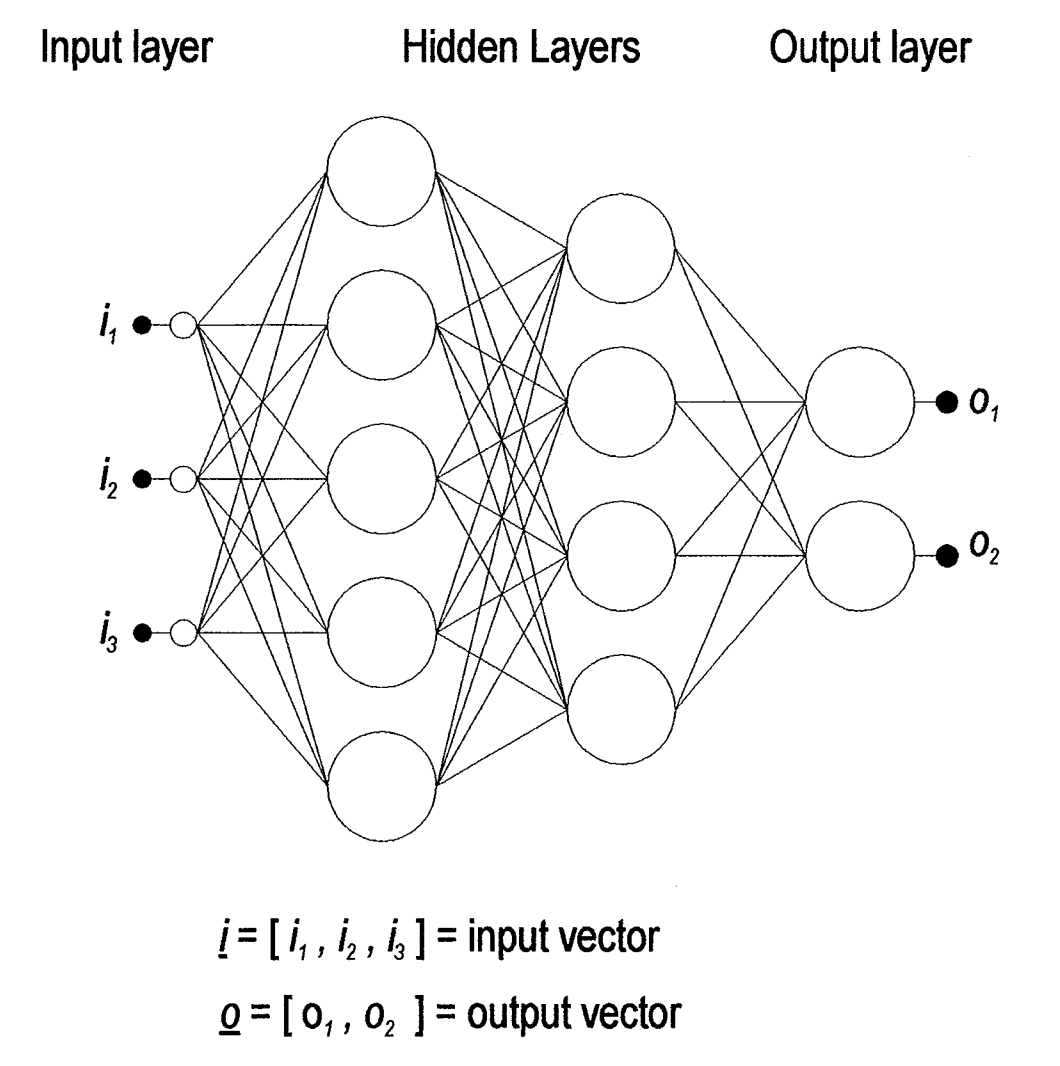
\includegraphics[width=8cm]{kapitel2/multilayerperc.png}
    \caption[Das mehrschichtige Perzeptron]{Das mehrschichtige Perzeptron mit zwei verborgenen Schichten, entnommen aus \cite*{Gardner1998}}
    
\end{figure}


\section{Sigmoid-Neuron}

Neben dem Perzeptron gibt es das Sigmoid Neuron. Das Perzeptron gibt bekannt nur eine 0 oder eine 1 zurück. Es ist also eine Funktion nötig, die sich ohne ohne Diskontinuität schrittweise von 0 auf 1 ändert. Mathematisch bedeutet dies, dass eine stetige Funktion nötig ist, mit der die Ableitung berechnet werden kann. Dieses Problem kann überwunden werden, indem einen neuer Typ eines künstlichen Neurons eingeführt wird, der als \textbf{Sigmoid-Neuron} bezeichnet wird. Sigmoid Neuronen ähneln Perzeptronen, sind jedoch so modifiziert, dass kleine Änderungen ihres Gewichts und ihres Bias nur eine geringe Änderung ihrer Leistung bewirken. Dies ist der Grund dafür, dass Netzwerke lernen können \cite*[8]{Nielsen2015}.

\begin{figure}[H]
    \centering
    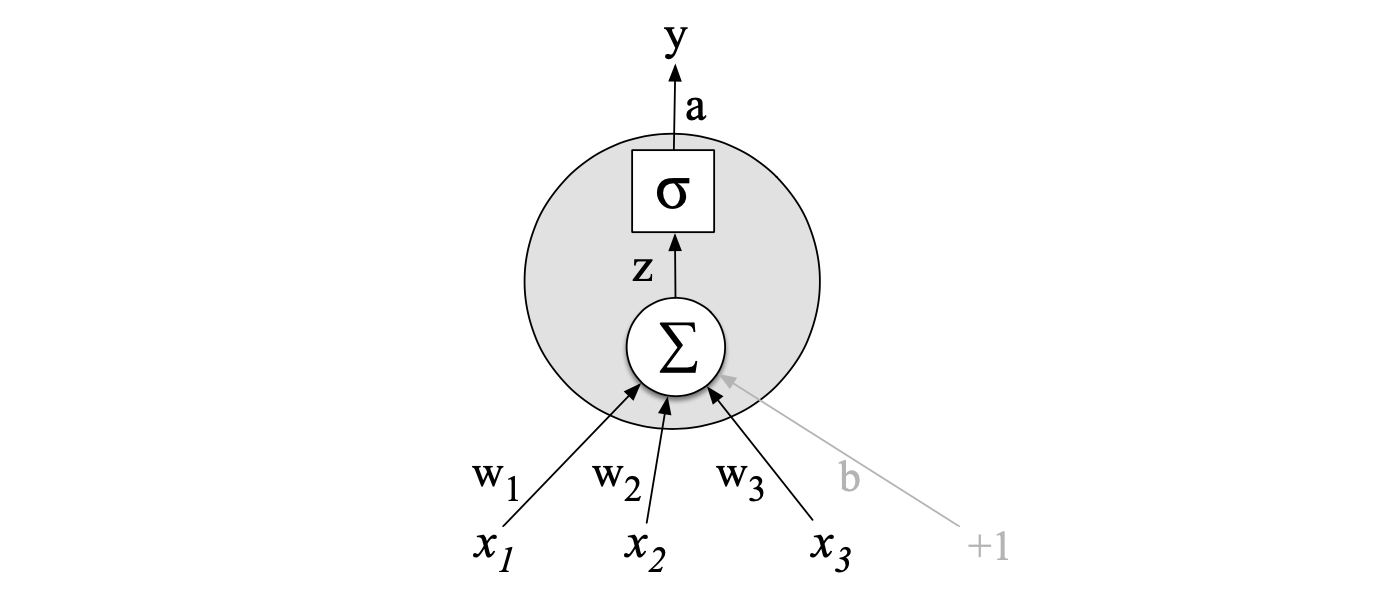
\includegraphics[width=11cm]{kapitel2/neuron.png}
    \caption[Eine neuronale Einheit]{Eine neuronale Einheit, die 3 Eingänge \textit{x1}, \textit{x2} und \textit{x3} (und eine Bias \textit{b}) einnimmt und einen Ausgang \textit{y} erzeugt. Durch Summieren entsteht \textit{z}. Das Sigmoid nimmt \textit{z} ein und erzeugt \textit{a}. In diesem Fall ist die Ausgabe \textit{y} dieselbe wie \textit{a}, aber in tiefen Netzwerken wird \textit{y} vorbehalten, um die endgültige Ausgabe des gesamten Netzwerks zu berechnen. Entnommen aus \cite[125]{Jurafskya}}
    \label{neurch2}
\end{figure}


Genau wie ein Perzeptron hat das Sigmoid-Neuron die Eingaben $x_1, x_2, ...$, aber anstatt nur 0 oder 1 zu sein, können diese Eingänge auch beliebige Werte zwischen 0 und 1 annehmen. Also zum Beispiel 0,123 welches eine gültige Eingabe für ein Sigmoid-Neuron ist. Ebenso wie ein Perzeptron hat das Sigmoid-Neuron Gewichte für jede Eingabe, $w_1, w_2, ...$ und einen Bias, $b$. Die Ausgabe ist jedoch nicht 0 oder 1, stattdessen ist es $\sigma$, $(wx + b)$, wobei $\sigma$ als Sigmoidfunktion bezeichnet wird und durch Formel~\ref{SigmoidFu} definiert ist.

\begin{equation} \label{SigmoidFu}
    \sigma (z) = \frac{1}{1+e^{-z}}
\end{equation}

\myequations{Sigmoidfunktion}


\section{Aktivierungsfunktionen}
Ohne eine \textbf{Aktivierungsfunktion} (auch als Nichtlinearität bezeichnet) würde die dichte Schicht (dense layer) nur aus zwei linearen Operationen bestehen - einem Punktprodukt und einer Addition: $Ausgabe = Punkt (w, Eingabe) + b$. Die Schicht konnte also nur lineare Transformationen (affine Transformationen) der Eingabedaten lernen. Um Zugang zu einem viel umfangreicheren Hypothesenraum zu erhalten, wird eine Nichtlinearitäts- oder Aktivierungsfunktion benötigt \cite*[S. 72]{Chollet2017}.

\subsection{Sigmoid}
Die Sigmoidfunktion wird mit der Formel~\ref{Formel2_2} definiert und in der Abbildung~\ref{Kap2:Sigmoid_plot} dargestellt, die Ableitung der Sigmoidfunktion wird in der Formel~\ref{AbleitungSigm} definiert. Sie hat kleine Ausgangsänderungen im Bereich (0, 1), wenn der Eingang im Bereich $(-\infty, \infty)$ variiert. Mathematisch ist die Funktion stetig. Ein Neuron kann das Sigmoid zur Berechnung der nichtlinearen Funktion $\sigma(z = wx + b)$ verwenden. Wenn $z = wx + b$ sehr groß und positiv wird, dann wird $e^z \rightarrow 0$ also $\sigma(z) \rightarrow 1$, während wenn $z = wx + b$ sehr groß und negativ wird, wird $e^{-z} \rightarrow 0$ also $\sigma(z) \rightarrow 0$. Mit anderen Worten, ein Neuron mit Sigmoidaktivierung hat ein ähnliches Verhalten wie das Perzeptron, aber die Änderungen sind allmählich und Ausgabewerte wie 0,54321 oder 0,12345 sind vollkommen legitim. In diesem Sinne kann ein Sigmoid-Neuron auch mit \enquote{vielleicht} antworten \cite*[10]{AntonioGuili;AmitaKapoor;SujitPal2019}.

\begin{figure}[H]
    \centering
    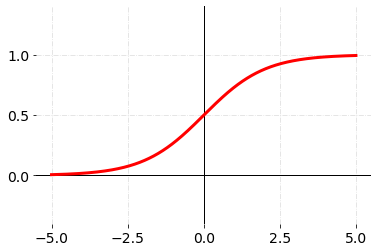
\includegraphics[width=8cm]{kapitel2/sig_plot.png}
    \caption[Darstellung der Sigmoid-Aktivierungsfunktion]{Darstellung der Sigmoid-Aktivierungsfunktion (eigene Darstellung)}
    \label{Kap2:Sigmoid_plot}
\end{figure}


\begin{equation} \label{AbleitungSigm}
    \begin{array}{ c }
        \sigma '(z)\ =\ \frac{d}{dz}\left(\frac{1}{1+e^{-z}}\right) =\frac{1}{\left( 1+e^{-z}\right)^{-2}}\frac{d}{dz} =\left( e^{-z}\right) \ =\frac{e^{-z}}{\left( 1+e^{-z}\right)}\frac{1}{\left( 1+e^{-z}\right)} \ =  \\
        \\
        \frac{e^{-z} +1-1}{\left( 1+e^{-z}\right)}\frac{1}{\left( 1+e^{-z}\right)} =\left(\frac{\left( 1+e^{-z}\right)}{\left( 1+e^{-z}\right)} -\frac{1}{\left( 1+e^{-z}\right)}\right)\frac{1}{\left( 1+e^{-z}\right)} = \\
        \\
        \left( 1-\frac{1}{\left( 1+e^{-z}\right)}\right)\left(\frac{1}{\left( 1+e^{-z}\right)}\right) =\ (1-\sigma (z))\sigma (z)
    \end{array}
\end{equation}
\label{AbleitungSigm}
\myequations{Ableitung der Sigmoidfunktion}

\subsection{Tanh}
Die Tanh-Aktivierungsfunktion wird mit der Formel~\ref{TanhF} definiert ihre Ableitung wird in der Formel~\ref{TanhAbl} berechnet. Sie hat ihre Ausgangsänderungen im Bereich (-1, 1). Sie hat eine Struktur, die der Sigmoid-Funktion sehr ähnlich ist. Der Vorteil gegenüber der Sigmoidfunktion besteht darin, dass ihre Ableitung steiler ist, was bedeutet, dass sie mehr Werte enthalten kann (vergleiche Abbildung~\ref{Kap2:Tanh_plot}). Für die Ableitung der Tanh-Aktivierungsfunktion gilt, $e^z = \frac{d}{dz}e^z$ und $e^{-z} = \frac{d}{dz}e^{-z}$.

\begin{equation} \label{TanhF}
    tanh(z) = \frac{e^{z}-e^{-z}}{e^{z}-e^{-z}}
\end{equation}
\myequations{Die Tanh-Funktion}

\begin{equation} \label{TanhAbl}
    \begin{array}{ c }
        \frac{d}{dz} tanh( x) =\frac{\left( e^{z} +e^{-z}\right)\left( e^{z} +e^{-z}\right) -\left( e^{z} -e^{-z}\right)\left( e^{z} -e^{-z}\right)}{\left( e^{z} +e^{-z}\right)^{2}} = \\
        \\
        1-\frac{\left( e^{z} -e^{-z}\right)^{2}}{\left( e^{z} +e^{-z}\right)^{2}} \ =\ 1\ -tanh^{2}( z)
    \end{array}
\end{equation}
\myequations{Die Ableitung der Tanh-Funktion}

\begin{figure}[H]
    \centering
    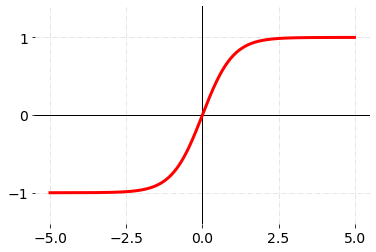
\includegraphics[width=8cm]{kapitel2/tanh_plot.png}
    \caption[Darstellung der Tanh-Aktivierungsfunktion]{Darstellung der Tanh-Aktivierungsfunktion (eigene Darstellung)}
    \label{Kap2:Tanh_plot}
\end{figure}

\subsection{ReLu}
Vor kurzem wurde eine sehr einfache Funktion namens ReLU (REctified Linear Unit) sehr beliebt, da sie dazu beiträgt, einige Optimierungsprobleme die bei Sigmoiden beobachtet werden, zu lösen \cite*[11]{AntonioGuili;AmitaKapoor;SujitPal2019}. Sie wird in Formel~\ref{Relu} definiert, die zugehörige Ableitungsfunktion wird in der Formel~\ref{ReluAbl} berechnet. Wie in Abbildung~\ref{Kap2:ReLu_plot} zu sehen, ist die Funktion für negative Werte Null und wächst für positive Werte linear. Die ReLU ist relativ einfach zu implementieren.

\begin{equation} \label{Relu}
    f( x) \ =\ \begin{cases}
        0 & wenn\ x\  <\ 0    \\
        x & wenn\ x\  \geq\ 0 \\
    \end{cases}
\end{equation}
\myequations{Die ReLu-Funktion}

\begin{equation} \label{ReluAbl}
    f'( x) \ =\ \begin{cases}
        1, & wenn\ x\  >\ 0 \\
        0, & sonst
    \end{cases}
\end{equation}
\myequations{Die Ableitung der ReLu-Funktion}

\begin{figure}[H]
    \centering
    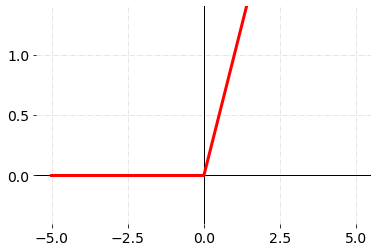
\includegraphics[width=8cm]{kapitel2/relu_plot.png}
    \caption[Darstellung der ReLu-Aktivierungsfunktion]{Darstellung der ReLu-Aktivierungsfunktion (eigene Darstellung)}
    \label{Kap2:ReLu_plot}
\end{figure}

\subsection{softmax}
Die grundlegende Schwierigkeit bei der Durchführung kontinuierlicher Mathematik auf einem digitalen Computer besteht darin, dass unendlich viele reelle Zahlen mit einer endlichen Anzahl von Bitmustern dargestellt werden müssen. Dabei entstehen Rundungsfehler die problematisch sein können, insbesondere wenn sie sich über viele Operationen hinweg zusammensetzen. Sieführen dazu, dass theoretisch funktionierende Algorithmen in der Praxis fehlschlagen. Ein Beispiel für eine Funktion, die gegen Rundungsfehler stabilisiert, ist die softmax-Funktion \cite*[80-81]{IanGoodfellowYoshuaBengio2016}.

\begin{equation} \label{FormelSoft}
    softmax( x)_{i} =\frac{exp( x_{i})}{\sum ^{n}_{j=1} exp( x_{j})}
\end{equation}
\myequations{Die softmax-Funktion}

\section{Optimierungsalgorithmen}
Die meisten Deep-Learning-Algorithmen beinhalten irgendeine Art von Optimierung. Optimierung bezieht sich auf die Aufgabe, eine Funktion $f(x)$ durch Ändern von $x$ entweder zu minimieren oder zu maximieren. Die meisten Optimierungsprobleme werden in Bezug auf Minimierung von $f(x)$ formuliert. Die Maximierung kann über einen Minimierungsalgorithmus durch Minimieren von $-$$f(x)$ erreicht werden. Die Funktion die minimiert oder maximiert werden soll, wird als \textbf{Objektive Funktion} bezeichnet. Es wird auch \textbf{Kostenfunktion} oder \textbf{Verlustfunktion} bezeichnet. Zum Beispiel ist die Funktion $x^{*} = arg\ min\ f( x)$ eine solche Funktion.

        \subsection{Gradientenverfahren}
        Der Gradientenabstieg ist einer der beliebtesten Algorithmen zur Optimierung und bei weitem der häufigste Weg zur Optimierung neuronaler Netze. Der Gradientenabstieg ist ein Weg, um eine Zielfunktion $J(\theta)$ zu minimieren, die durch die Parameter eines Modells $\theta \in \mathbb{R}^{d}$ parametrisiert wird. Die Parameter werden in der entgegengesetzten Richtung des Gradienten der Zielfunktion $\nabla \theta J (\theta)$ angepasst. Die Lernrate $\eta$ bestimmt die Größe der Schritte, die unternommen werden, um ein lokales Minimus zu erreichen. Mit anderen Worten, wird der Richtung bergab gefolgt, die durch die Zielfunktion erzeugt wird, bis ein \enquote{Tal} erreicht wird (siehe Abbildung~\ref{Kap2:Grad}) \cite*{Ruder2016}.



        \begin{figure}[H]
            \centering
            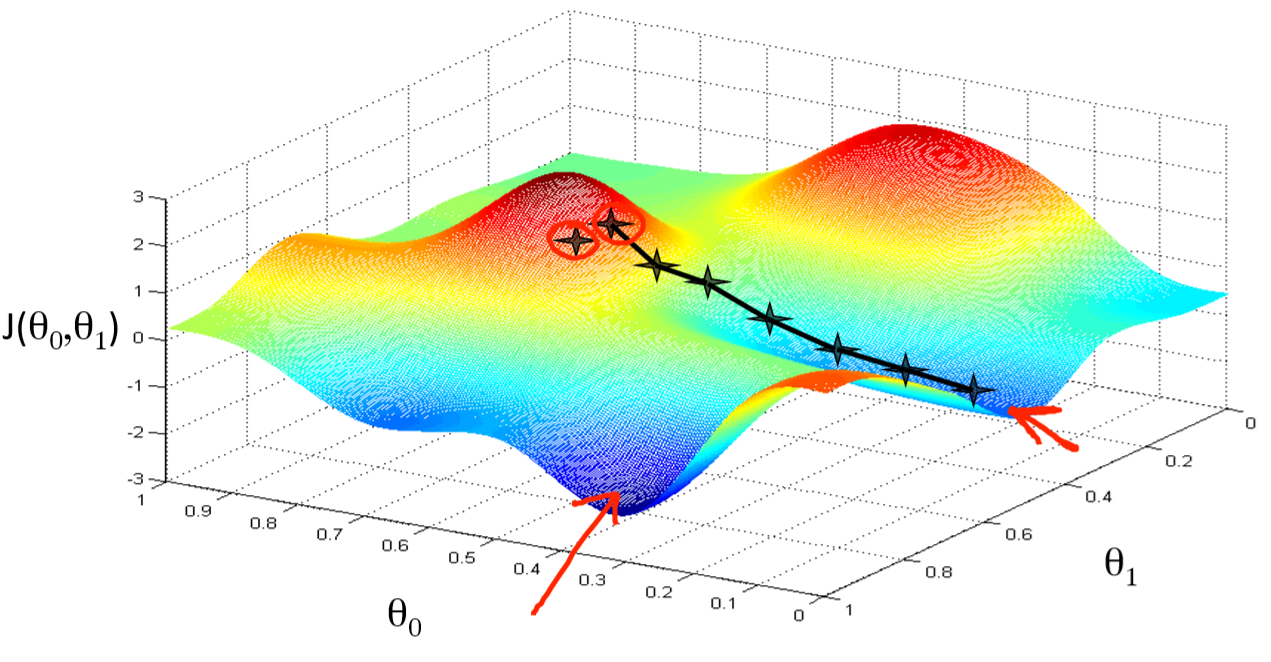
\includegraphics[width=12cm]{kapitel2/gradient.png}
            \caption[Der Gradientenabstieg]{Darstellung des Gradientenabstiegs, entnommen aus \cite*{hackernoon}.}
            \label{Kap2:Grad}
        \end{figure}



        \subsection{Batch Gradientenabstiegsverfahren}
        Der Standart Gradientenabstiegsverfahren, auch Batch Gradientenabstiegsverfahren genannt, berechnet den Gradienten der Verlustfunktion zu den Parametern $\theta$ für den gesamten Trainingsdatensatz.


        \begin{equation} \label{FormelGradBatch}
            \theta = \theta - \eta \cdot \nabla_{\theta}J(\theta)
        \end{equation}
        \myequations{Die Gradientensteigung}

        Da der gesamte Datensatz berechnet werden muss, um nur eine Aktualisierung durchzuführen, kann der Batch Gradientenabstieg sehr langsam sein und ist für Datensätze, die nicht in den Speicher passen, nicht zu handhaben. Der Batch Gradientenabstieg ermöglicht es auch nicht, das Modell mit neuen Beispielen im laufenden Betrieb zu aktualisieren \cite*{Ruder2016}.

        \subsection{Stochastische Gradientenabstiegsverfahren}

        Im Gegensatz dazu führt der stochastische Gradientenabstiegsverfahren (SGD) eine Parameteraktualisierung für jedes Trainingsbeispiel durch. Der Batch Gradientenabstieg führt redundante Berechnungen für große Datenmengen durch, da Gradienten für ähnliche Beispiele vor jeder Parameteraktualisierung neu berechnet werden. Der Stochastische Gradientenabstiegsverfahren beseitigt diese Redundanz, indem jeweils ein Update durchgeführt wird. Es ist daher in der Regel viel schneller und kann auch beim laufendem Lernen verwendet werden \cite*{Ruder2016}.

        \begin{equation} \label{FormelGradStoch}
            \theta = \theta - \eta \cdot \nabla_{\theta}J(\theta;x^{(i)};y^{(i)})
        \end{equation}
        \myequations{Die stochastische Gradientensteigung}



        \section{Backpropagation}
        Das \textbf{Backpropagation} Verfahren bezieht sich auf die Gewichte eines mehrschichtigen Netzes und wendet dabei praktisch die Anwendung der Kettenregel der  Differentialrechnung an. Es wird vom Gradienten in Bezug auf die Ausgabe (oder die Eingabe der Nachfolge) rückwärts gearbeitet. Die Kettenregel sagt dabei aus, wie zwei kleine Effekte (eine kleine Änderung von $x$ auf $y$ und der von $y$ auf $z$) zusammengesetzt sind. Eine kleine Änderung von $\Delta y$ in $x$ wird zuerst in eine kleine Änderung $\Delta y$ in $y$ umgewandelt, indem sie mit $\frac{\partial y}{\partial y}$  multipliziert wird (die partielle Ableitung). In ähnlicher Weise erzeugt die Änderung $\Delta y$ eine Änderung von $\Delta z$ in $z$ (siehe Formel~\ref{ChainRule}) \cite*{Lecun2015}.

        \begin{gather} \label{ChainRule}
            \Delta z =  \frac{\partial z}{\partial y} \Delta y \notag\\
            \Delta y = \frac{\partial y}{\partial x} \Delta x \notag\\
            \Delta z = \frac{\partial z}{\partial y}\frac{\partial y}{\partial x} \Delta x \notag\\
            \frac{\partial z}{\partial x} = \frac{\partial z}{\partial y} \frac{\partial y}{\partial x}
        \end{gather}
        \myequations{Backpropagation}




        Die Gleichungen, die zur Berechnung des \textbf{Vorwärtsdurchlaufs} (siehe Abbildung~\ref{BackProp}) in einem neuronalen Netz mit zwei verborgenen Schichten und einer Ausgangsschicht verwendet werden, bilden jeweils ein Modul, durch das man Gradienten zurückpropagieren kann. Auf jeder Ebene wird zuerst die Gesamteingabe $z$ für jede Einheit berechnet. Dann wird eine nichtlineare Funktion auf $z$ angewendet, um die Ausgabe der Einheiten zu erhalten (der Bias wurde hier der Einfachheit halber weggelassen). Eine nichtlineare Funktion kann z.B. eine ReLu- oder eine Sigmoid-Funktion oder eine tanh-Funktion sein. Im \textbf{Rückwärtsdurchlauf} (siehe Abbildung~\ref{BackProp}) wird in jeder verborgenen Schicht die Fehlerableitung in Bezug auf die Ausgabe jeder Einheit berechnet. Dies geschieht durch Vergleichen der Ausgaben mit der richtigen Antwort, um Fehlerableitungen zu erhalten \cite*{Lecun2015}.


        \begin{figure}[H]
            \centering
            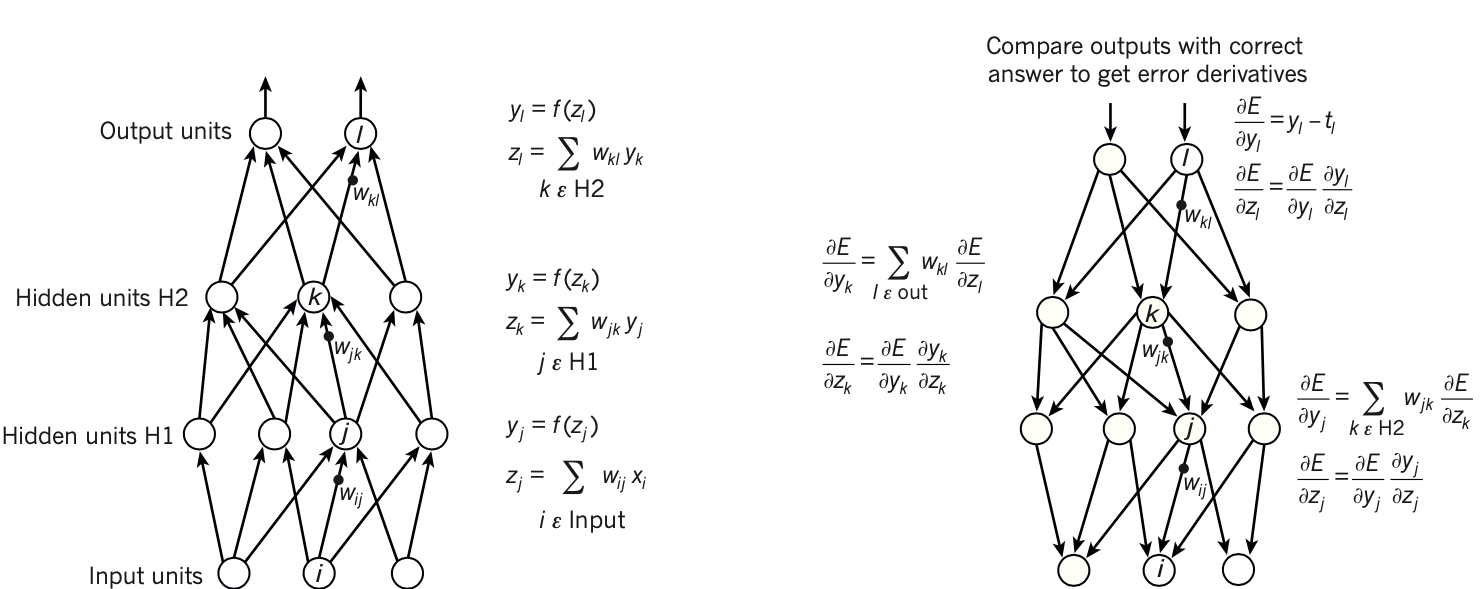
\includegraphics[width=13cm]{kapitel2/backprop.png}
            \caption[Die Vorwärts- und Rückwärtsschritte im Backpropagation]{Darstellung vergleicht die Schritte des Backpropagation Verfahrens nach vorne und hinten (in Anlehnung an \cite*{Lecun2015}).}
            \label{BackProp}
        \end{figure}

        Die Backpropagation-Gleichung wird wiederholt angewendet. Der Rückwärtsdurchlauf bezieht sich auf die Idee, die Differenz zwischen Vorhersage- und Istwerten zu verwenden, um die Hyperparameter der verwendeten Methode anzupassen. Für die Anwendung ist jedoch immer eine vorherige Vorwärtspropagation erforderlich.


        \section{Lernrate im Deep Learning}\label{learnsection}
        Die \textbf{Lernrate} beeinflusst den Betrag, um den die Parameter während der Optimierung angepasst werden, um den Fehler des neuronalen Netzwerks zu minimieren. Es ist ein Koeffizient, der die Größe der Schritte (Aktualisierungen) skaliert, die ein neuronales Netzwerk auf seinen Parameter (Vektor $x$) ausführt, wenn es den Verlustfunktionsraum durchquert. Ein großer Lernratenkoeffizient (z. B. 1) lässt die Parameter Sprünge machen, und kleine (z. B. 0,00001) lassen ihn langsam voranschreiten. Im Gegensatz dazu sollten kleine Lernraten letztendlich zu einem Fehlerminimum führen (es kann eher ein lokales als ein globales Minimum sein). Sehr kleine Lernraten können sehr lange dauern und die Belastung eines bereits rechenintensiven Prozesses erhöhen  \cite*[77]{Patterson2019}.


        \begin{figure}[H]
            \centering
            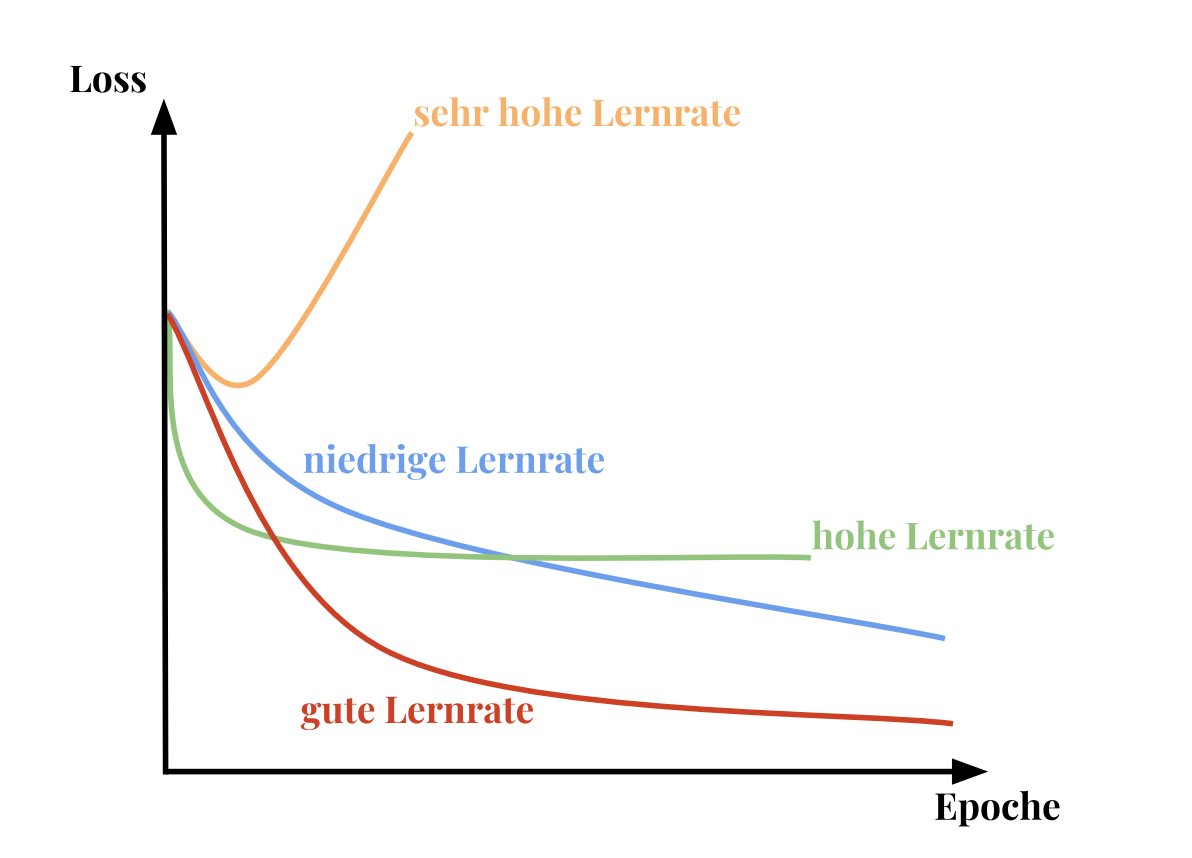
\includegraphics[width=10cm]{kapitel2/learnrate.png}
            \caption[Einfluss der Lernrate auf den Verlust]{Vergleich unterschiedlicher Lernraten und deren Effekt auf den Verlust. Bei niedrigen Lernraten ist eine \enquote{lineare} Verbesserungen zu sehen. Mit hohen Lernraten werden sie exponentieller. Höhere Lernraten verringern den Verlust schneller, bleiben jedoch bei schlechteren Verlustwerten hängen (grüne Linie). Dieses liegt daran, dass die Optimierung zu viel \enquote{Energie} enthält und die Parameter \enquote{chaotisch herumspringen} und sich nicht an einem Ort in der Optimierungslandschaft niederlassen können (in Anlehnung an \cite*{StanfordUniversityCoursecs231n2018}). }
            \label{Kap2:Lern}
        \end{figure}

        \section{Unteranpassung und Überanpassung}\label{overundersec}
        Optimierungsalgorithmen versuchen zunächst, das Problem der \textbf{Unteranpassung} \enquote{Underfitting} zu lösen. Das heißt, eine Linie zu nehmen, die sich den Daten nicht gut annähert, und sie besser an die Daten heranzuführen. Eine gerade Linie, die über ein gekrümmtes Streudiagramm schneidet, wäre ein gutes Beispiel für eine Unteranpassung, wie in Abbildung~\ref{Kap2:OverUnder} dargestellt. Wenn die Linie zu gut zu den Daten passt, haben wir das gegenteilige Problem, welches als \textbf{Überanpassung} \enquote{Overfitting} bezeichnet wird \cite*[27]{Patterson2019}.

        \begin{figure}[H]
            \centering
            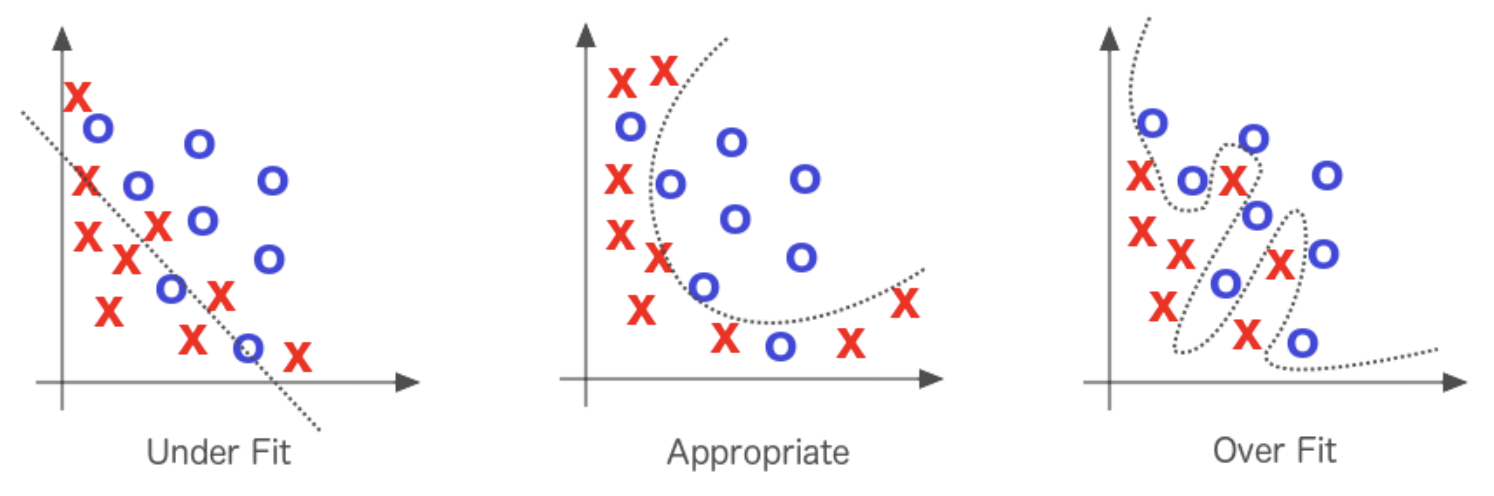
\includegraphics[width=10cm]{kapitel2/overundefit.png}
            \caption[Vergleich der Unteranpassung mit der Überanpassung]{Die Abbildung vergleicht die Überanpassung mit der Unteranpassung. Die einzelnen Punkte passen sich dem trainierten Model zu sehr an, der Verlust wird also so klein, dass das Modell nicht mehr zuverlässige Ergebnisse liefern kann. Dies ist darauf zurückzuführen, dass das Modell \enquote{zu viel} aus dem Trainingsdatensatz gelernt hat. Unteranpassung ist der Fall, wenn das Modell aus den Trainingsdaten \enquote{nicht genug gelernt} hat, was zu einer geringen Verallgemeinerung und unzuverlässigen Vorhersagen führt (Grafik entnommen aus \cite*[27]{Patterson2019}). }
            \label{Kap2:OverUnder}
        \end{figure}

        \section{Regularisierung}\label{regSec}
        Die Regularisierung lässt die Auswirkungen von außer Kontrolle geratenen Parametern minimieren, indem verschiedene Methoden oder Strategien verwendet werden, um die Parametergröße im Laufe der Zeit zu minimieren. Der Hauptzweck der Regularisierung besteht darin, die Überanpassung zu kontrollieren \cite*[79]{Patterson2019}.

        Ein zentrales Problem beim maschinellen Lernen besteht darin, einen Algorithmus zu erstellen, der nicht nur bei den Trainingsdaten, sondern auch bei neuen Eingaben eine gute Leistung erbringt. Viele beim maschinellen Lernen verwendete Strategien sind explizit darauf ausgelegt, den Testfehler zu reduzieren, möglicherweise auf Kosten eines erhöhten Trainingsfehlers. Diese Strategien werden zusammen als Regularisierung bezeichnet. Tatsächlich war die Entwicklung effektiverer Regularisierungsstrategien eine der wichtigsten Forschungsanstrengungen auf diesem Gebiet. Regularisierung kann schließlich definiert werden als \enquote{jede Änderung, die wir an einem Lernalgorithmus vornehmen, um dessen Generalisierungsfehler, aber nicht seinen Trainingsfehler zu reduzieren} \cite*[228]{IanGoodfellowYoshuaBengio2016}.

        \subsection{Early Stopping}
        Wenn große Modelle trainiert werden, um eine bestimmte Aufgabe lösen, wird häufig festgestellt, dass der Trainingsfehler mit der Zeit stetig abnimmt, der Fehler des Validierungssatzes jedoch wieder zunimmt. Dies bedeutet, dass ein Modell mit einem besseren Validierungssatzfehler (und damit einem besseren Testsatzfehler) erhalten werden kann, indem zu dem Zeitpunkt mit dem niedrigsten Validierungssatzfehler zur Parametereinstellung zurückgekehrt wird. Jedes Mal, wenn sich der Fehler im Validierungssatz verbessert, wird eine Kopie der Modellparameter gespeichert. Wenn der Trainingsalgorithmus beendet wird, wird diese Parameter anstelle der neuesten Parameter zurückgegeben. Diese Strategie wird als \textbf{Early Stopping} \enquote{frühes Stoppen} bezeichnet. Es ist wahrscheinlich die am häufigsten verwendete Form der Regularisierung. Seine Popularität ist sowohl auf seine Wirksamkeit als auch auf seine Einfachheit zurückzuführen \cite*[246]{IanGoodfellowYoshuaBengio2016}.


        \subsection{Dropout}
        Eine weitere Strategie um Überanpassung zu vermeiden wird in \cite*{Srivastava2014} dargestellt. \textbf{Dropout} bietet eine rechnerisch kostengünstige, aber leistungsstarke Methode zur Regularisierung dar. Es ist das aufteilen des Netzwerkes in mehreren Teile. Es wird also ein Ensemble aus diesen kleinen Teilen (sub-networks) gebildet \cite*[258]{IanGoodfellowYoshuaBengio2016}.



        \begin{figure}[H]
            \centering
            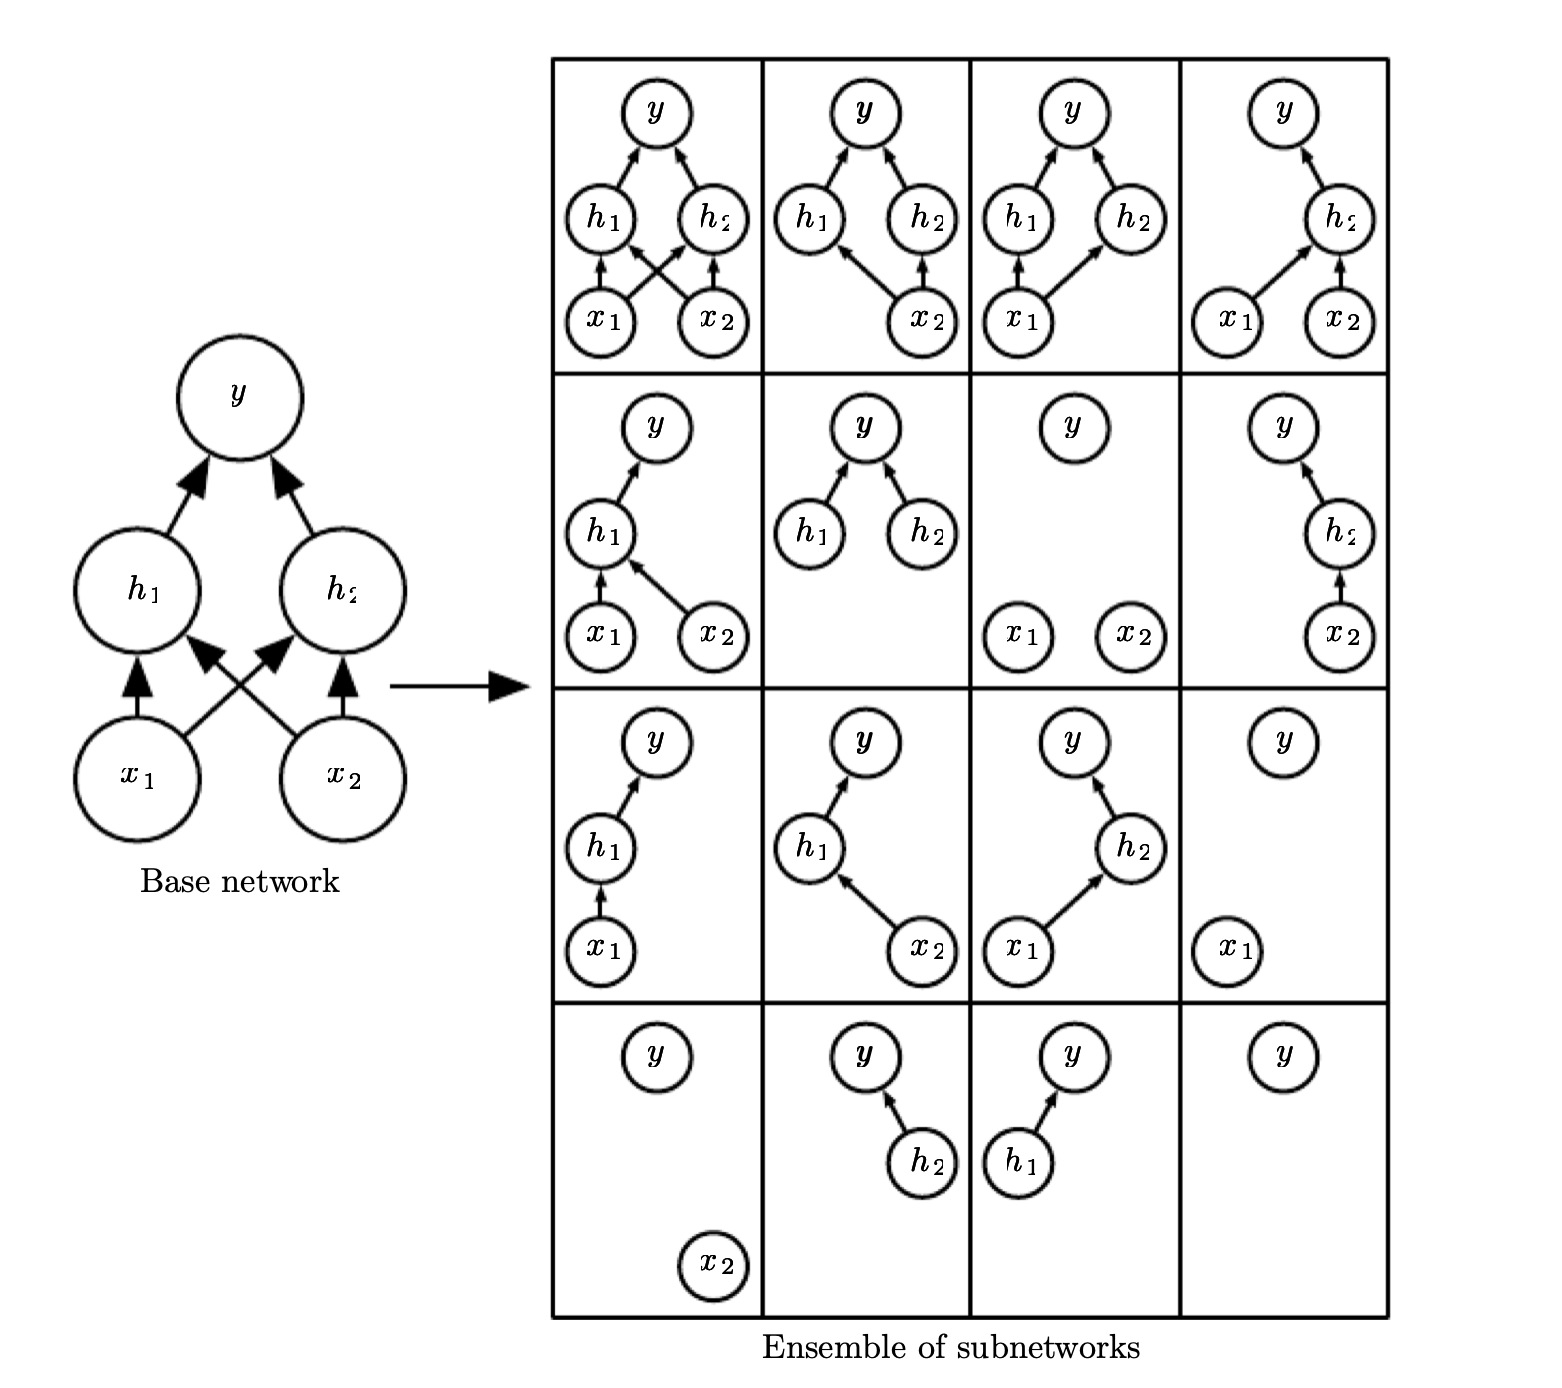
\includegraphics[width=10cm]{kapitel2/dropout.png}
            \caption[Basis-Netzwerks und Ensemble im Vergleich]{Dropout trainiert ein Ensemble. Ein Ensemble besteht aus allen Teilnetzwerken. Es wird durch das entfernen von Einheiten aufgebaut. Das Ensemble besteht aus 16 Teilmengen, aus den vier Einheiten des Basis-Netzwerks. Die 16 Subnetze werden durch das Löschen verschiedener Teilmengen von Einheiten aus dem ursprünglichen Netzwerk gebildet (entnommen aus \cite*[260]{IanGoodfellowYoshuaBengio2016}).}
            \label{Kap2:Dropout}
        \end{figure}

        \subsection{L1 und L2}
        Eine weitere Strategie der Regularisierung ist die Modifikation der L1 und L2 Gewichte. Beim Deep Learning wird die Größe von Vektoren mit einer Funktion, die als \enquote{Norm} bezeichnet wird \cite*[39]{IanGoodfellowYoshuaBengio2016} gemessen. Formal ist diese Norm $L^p$ gegeben als:

        \begin{equation} \label{FormelNorm2}
            \Vert x\Vert \ =\ \left(\sum _{i}\bigr| x_{i}\bigr|^{p}\right)^{\frac{1}{p}}.
        \end{equation}
        \myequations{Regularisierung}

        Normen, einschließlich der $L^p$-Norm, sind Funktionen, die Vektoren auf nicht negative Werte abbilden. Auf einer intuitiven Ebene misst die Norm eines Vektors $x$ den Abstand vom Ursprung zum Punkt $x$. Die $L^2$-Norm mit $p = 2$ als euklidische Norm bekannt. Es ist der euklidische Abstand vom Ursprung zum Punkt $x$. Die $L^2$-Norm wird beim maschinellen Lernen häufig verwendet, sie wird einfach als $\Vert x\Vert$ bezeichnet, wobei der Index 2 weggelassen wird \cite*[39]{IanGoodfellowYoshuaBengio2016}.

        Wenn zwischen Elementen zu unterscheiden ist, die genau Null sind und Elementen die klein, aber ungleich Null sind, wird die $L^1$-Norm angewendet. Die $L^1$-Norm kann vereinfacht werden als \cite*[40]{IanGoodfellowYoshuaBengio2016}:

        \begin{equation} \label{FormelNorm1}
            \Vert x\Vert 1\ =\ \sum _{i}\bigr| x_{i}\bigr|.
        \end{equation}
        \myequations{L1-Regularisierung}

\section{Metriken im Deep Learning}
Im Deep Learning werden oftmals Klassifizierungsprobleme gelöst. In diesem Abschnitt werden die wichtigsten Metriken für das Messen solcher Modelle definiert.
\paragraph{Precision}
Präzision gibt die Häufigkeit an, mit der ein Modell bei der Vorhersage der positiven Klasse korrekt war. Das ist:

\begin{equation} \label{Preci}
             Precision =  \frac{True\ Positives}{True\ Positives\ + False\ Positives}.
        \end{equation}
        \myequations{Precision}
\paragraph{Recall}
Ist eine Metrik, die die folgende Frage beantwortet: Wie viele der möglichen positiven Bezeichnungen hat das Modell korrekt identifiziert? Es wird definiert durch:
\begin{equation} \label{Recall}
             Recall =  \frac{True\ Positives}{True\ Positives\ + False\ Negatives}.
        \end{equation}
        \myequations{Recall}


\paragraph{F1-Score}
Der F1-Score ist das harmonische Mittel der Präzision und des Rückrufs. Es wird mit folgender Formel berechnet:
\begin{equation} \label{F1Score}
             F_1 =  2 \cdot \frac{Precision\ \cdot Recall}{Precision\  + Recall}.
        \end{equation}
        \myequations{F1-Score}
        

        \section{Verlustfunktion und Kreuzentropie}
        \subsection{Verlustfunktionen}
        Innerhalb eines neuronalen Netzwerks wandelt eine \textbf{Verlustfunktion} oder \textbf{Kostenfunktion} alle möglichen Fehler, in eine Zahl um, die den Gesamtfehler des Netzwerks darstellt. Im Wesentlichen ist es ein Maß dafür, wie falsch ein Netzwerk liegt.

        Das Neuron lernt dadurch, indem es Gewichte und Bias mit einer Rate ändert, die durch die partiellen Ableitungen der Kostenfunktion $\partial$$C$/$\partial$$w$ und $\partial$$C$/$\partial$$b$ bestimmt wird. Zu sagen, dass das \enquote{Lernen langsam ist}, ist also dasselbe wie zu sagen, dass diese partiellen Ableitungen klein sind \cite*[61]{Nielsen2015}. Gegeben sei die quadratische Verlustfunktion:

        \begin{equation} \label{Formel2_5}
            C=\frac{( y-a)^{2}}{2},
        \end{equation}
        \myequations{Kostenfunktion}

        dabei ist $a$ die Ausgabe des Neurons, wenn die Trainingseingabe $x = 1$ ist, und $y = 0$ die entsprechende gewünschte Ausgabe. Um dies in Bezug auf Gewicht und Bias expliziter zu schreiben, sei daran erinnert, dass $a = \sigma(z)$ ist, wobei $z = wx + b$ ist. Es ergeben sich durch die Anwendung der Kettenregel folgende Gleichungen:

        \begin{equation} \label{Formel2_6}
            \frac{\partial C}{\partial w} =( a-y) \sigma '( z) x=a\sigma '( z)
        \end{equation}
        \myequations{Partielle Kostenfunktion der Gewichte}

        \begin{equation} \label{Formel2_7}
            \frac{\partial C}{\partial b} =( a-y) \sigma '( z) =a\sigma '( z).
        \end{equation}
        \myequations{Partielle Kostenfunktion des Bias}
        
        Aus der Abbildung~\ref{Kap2:Sigmoid_plot} ist die Kurve der Sigmoidfunktion zu sehen. Die Kurve wird sehr flach, wenn der Ausgang des Neurons nahe bei 1 liegt, und daher wird $\sigma'(z)$ sehr klein. Die Gleichungen~\ref{Formel2_6} und ~\ref{Formel2_7} sagen dann aus, dass $\partial$$C$/$\partial$$w$  und  $\partial$$C$/$\partial$$b$ sehr klein werden. Dies ist der Grund warum das lernen langsamer wird.

    \subsection{Kreuzentropie}
    Nach \cite*[62]{Nielsen2015} kann die Lernverlangsamung gelöst werden, indem die quadratische Verlustfunktion durch eine andere Verlustfunktion ersetzt wird. Diese Funktion wird als als \textbf{Kreuzentropie} bezeichnet. Die Abbildung~\ref{Kap2:Entropie} zeigt die Kreuzentropie mit mehreren Eingabevariablen und entsprechenden Gewichten und dem Bias. Die Ausgabe des Neurons ist $a = \sigma(z)$, wobei $z =  \sum _{j} w_{j} b_{j} + b$ ist, die gewichtete Summe des Inputs. Die Kreuzentropiekostenfunktion für dieses Neuron wird definiert durch:

    \begin{equation} \label{Formel2_8}
        C=\ -\frac{1}{n}\sum _{x}[ y\ ln\ a\ +\ ( 1-y) \ ln( 1-a)]
    \end{equation}
    \myequations{Kreuzentropie}

    wobei $n$ die Gesamtzahl der Trainingselemente darstellt. Die Summe gibt die entsprechende gewünschte Ausgabe $x$ und $y$ über alle Trainingseingaben an. Zusammenfassend ist die Kreuzentropie positiv und tendiert gegen Null, wenn das Neuron
    \enquote{besser} wird in der Berechnung der gewünschten Ausgabe $y$ für alle Trainingseingaben $x$ ist.  Die entropieübergreifende Kostenfunktion hat jedoch den Vorteil, dass sie im Gegensatz zu den quadratischen Kosten das Problem der Verlangsamung des Lernens vermeidet. Um dies zu sehen, wird die partielle Ableitung der Kreuzentropiekosten in Bezug auf die Gewichte berechnet \cite*[63]{Nielsen2015}.

    \begin{gather} \label{Formel2_9}
        \frac{\partial C}{\partial w_{j}} =-\frac{1}{n}\sum _{x}\left(\frac{y}{\sigma ( z)} -\frac{1-y}{1-\sigma ( z)}\right)\frac{\partial \sigma }{\partial w_{j}} = \notag\\
        -\frac{1}{n}\sum _{x}\left(\frac{y}{\sigma ( z)} -\frac{1-y}{1-\sigma ( z)}\right) \sigma '( z) x_{j}
        \notag\\
        \frac{\partial C}{\partial w_{j}} \ =\ \frac{1}{n}\sum _{x}\frac{\sigma '( z) x_{j}}{\sigma ( z)( 1-\sigma ( z))}( \sigma ( z) -y)
        \notag\\
        \frac{\partial C}{\partial w_{j}} \ =\ \frac{1}{n}\sum _{x} x_{j}( \sigma ( z) -y)
    \end{gather}
    \myequations{Herleitung der Kreuzentropie}

    Die Geschwindigkeit, mit der das Gewicht $w$ lernt, wird durch $\sigma(z) - y$ gesteuert, also durch den Fehler in der Ausgabe. Je größer dieser Fehler wird, desto schneller lernt das Neuron. Dies ist ein gewünschtes Verhalten. Insbesondere wird die Lernverlangsamung vermieden, die durch den Term $\sigma'(z)$ in der analogen Gleichung für die quadratischen Kostenfunktion~\ref{Formel2_6} verursacht wird. Wenn die Kreuzentropie verwendet wird, wird der Term $\sigma'(z)$ aufgehoben und somit ist es egal, ob es klein ist. Diese Aufhebung ist das Besondere, welches durch die Kreuzentropie-Kostenfunktion gewährleistet wird \cite[63-64]{Nielsen2015}.

    \begin{figure}[H]
        \centering
        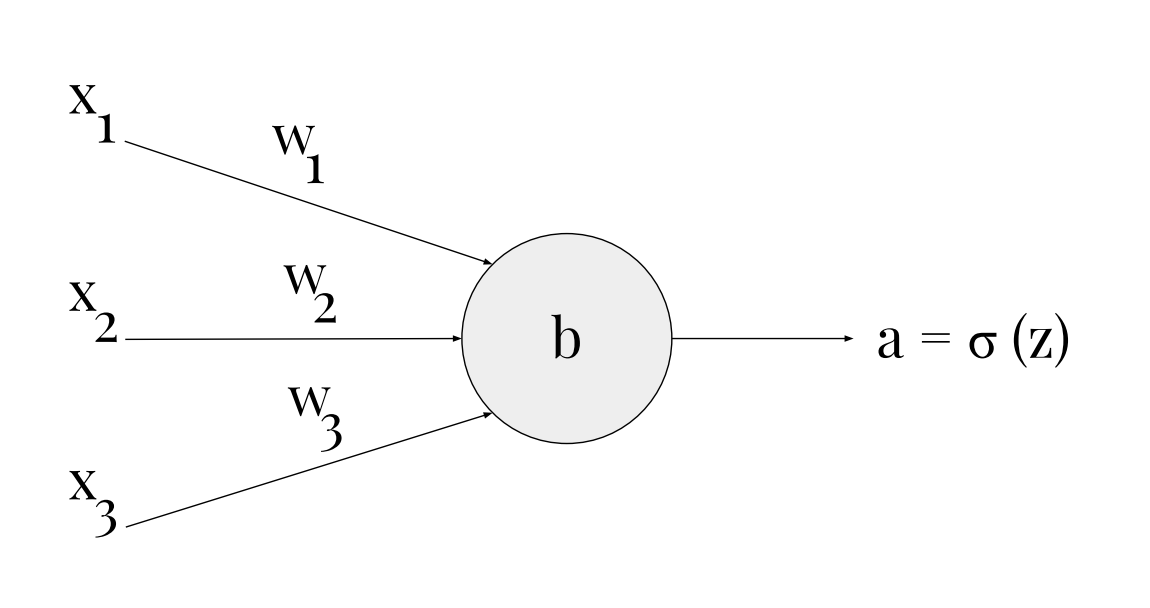
\includegraphics[width=8cm]{kapitel2/entropie.png}
        \caption[Darstellung der Kreuzentropie am beispiel eines Neurons]{Das Neuron wird mit 3 Eingabewerten $(x_1, x_2, x_3)$ den dazugehörigen Gewichten $(W_1, W_2, W_3)$ trainiert. Der Bias ist durch $b$ angegeben und die Ausgabe mit $a = \sigma(z)$ (in Anlehnung an \cite*{Nielsen2015})}
        \label{Kap2:Entropie}
    \end{figure}

    \section{Convolutional Neural Network}

    ConvNets/CNNs oder \textbf{Convolutional Neural Networks} dienen zur Verarbeitung von Daten in Form mehrerer Arrays, beispielsweise eines Farbbilds aus drei 2D-Arrays mit Pixelintensitäten in den drei Farbkanälen. Viele Datenmodalitäten liegen in Form mehrerer Arrays vor: 1D für Signale und Sequenzen, einschließlich Sprache; 2D für Bilder oder Audiospektrogramme; und 3D für Video- oder Volumenbilder. Hinter ConvNets stehen vier Schlüsselideen, die die Eigenschaften natürlicher Signale nutzen: lokale Verbindungen, gemeinsame Gewichte, Pooling und die Verwendung vieler Schichten \cite*{Lecun2015}.


    CNNs arbeiten mit gitterstrukturierten Eingaben, die in lokalen Regionen des Netzes starke räumliche Abhängigkeiten aufweisen. Das offensichtlichste Beispiel für gitterstrukturierte Daten ist ein zweidimensionales Bild. Diese Art von Daten weisen räumliche Abhängigkeiten auf, da benachbarte räumliche Orte in einem Bild häufig ähnliche Farbwerte der einzelnen Pixel aufweisen. Eine zusätzliche Dimension erfasst die verschiedenen Farben, wodurch ein dreidimensionales Eingabevolumen entsteht. Andere Formen von sequentiellen Daten wie Text, Zeitreihen und Sequenzen können ebenfalls als Sonderfälle von Daten mit Gitterstruktur mit verschiedenen Arten von Beziehungen zwischen benachbarten Elementen betrachtet werden. Die überwiegende Mehrheit der Anwendungen von CNNs konzentriert sich auf Bilddaten, obwohl man diese Netze auch für alle Arten von zeitlichen, räumlichen und raumzeitlichen Daten verwenden kann. Ein wichtiges definierendes Merkmal von CNNs ist eine Operation, die als Faltung (convolution) bezeichnet wird. \cite*[315-316]{Aggarwal2018}.




    \subsection{Architektur}
    In CNNs sind mehrere Schichten miteinander verbunden und jeder Schicht hat eine Gitterstruktur. Die Bezihungen zwischen den Schichten werden von einer Schicht zur nächsten vererbt, da jeder Merkmalswert auf einem kleinen lokalen Bereich aus der vorherigen Schicht basiert. Es ist wichtig, diese räumlichen Beziehungen zwischen den Gitterzellen aufrechtzuerhalten, da die Faltungsoperation und die Transformation zur nächsten Schicht von diesen Beziehungen abhängen. Jede Schicht im Faltungsnetzwerk ist eine dreidimensionale Gitterstruktur mit einer Höhe, Breite und Tiefe. Die Tiefe einer Schicht in einem Faltungsnetzwerk ist nicht die Tiefe des Netzwerks selbst. Das Wort \enquote{Tiefe} bezieht sich auf die Anzahl der Kanäle in jeder Ebene, z. B. die Anzahl der Primärfarbkanäle (z. B. Blau, Grün und Rot) im Eingabebild \cite*[318]{Aggarwal2018}.

    Die Architektur eines typischen ConvNets ist in mehrere Phasen unterteilt. Die ersten Stufen bestehen aus zwei Arten von Schichten: Faltungsschichten und Poolschichten. Einheiten in einer Faltungsebene sind in \textbf{Feature-Maps} organisiert, in denen jede Einheit über eine Reihe von Gewichten, die als Filterbank bezeichnet werden, mit lokalen Patches in den Feature-Maps der vorherigen Ebene verbunden ist. Das Ergebnis dieser lokal gewichteten Summe wird dann durch eine Nichtlinearität wie \zb eine ReLU geleitet. Alle Einheiten in einer Feature-Map verwenden dieselbe Filterbank\cite*{Lecun2015}.


    \begin{figure}[H]
        \centering
        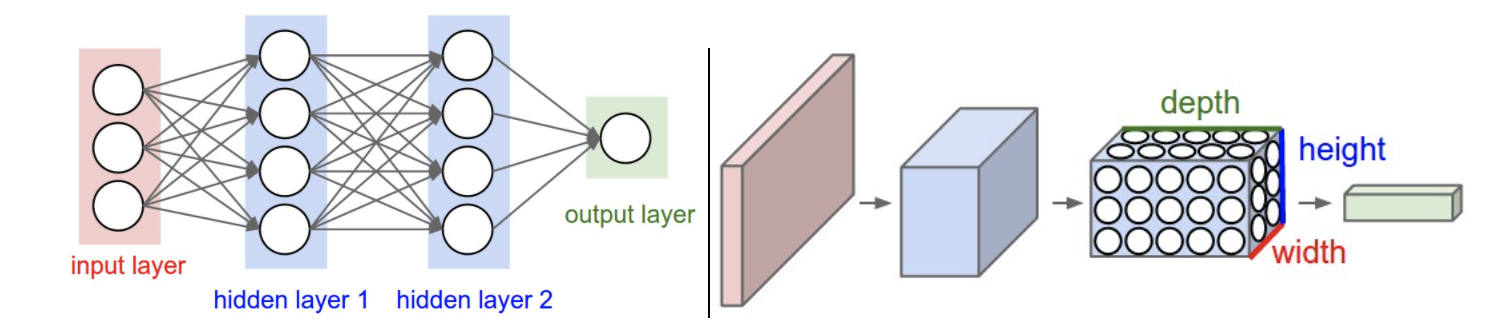
\includegraphics[width=13cm]{kapitel2/conv.png}
        \caption[Vergleich eines NN mit einem CNN]{Links: Ein reguläres 3-Schicht-Neuronales Netz. Rechts: Ein ConvNet ordnet seine Neuronen in drei Dimensionen (Breite, Höhe, Tiefe) an, wie in einer der Ebenen dargestellt. Jede Schicht eines ConvNet wandelt das 3D-Eingangsvolumen in ein 3D-Ausgangsvolumen von Neuronenaktivierungen um. In diesem Beispiel enthält die rote Eingabeebene das Bild, sodass seine Breite und Höhe den Abmessungen des Bildes entsprechen. Die \enquote{Tiefe} sind die 3 Farbkanäle (rot, grün, blau) aus \cite*{StanfordUniversityCoursecs231n2018a}.}
        \label{Kap2:Conv}
    \end{figure}


    \subsection{Convolutional Layer}

    Die Parameter der  \textbf{Convolutional Layer} oder \textbf{Faltungsschicht} bestehen aus einer Reihe von lernbaren Filtern. Jedes dieser Filter ist räumlich klein (Breite und Höhe), erstreckt sich jedoch über die gesamte Tiefe des Eingangsvolumens. Beispielsweise könnte ein typischer Filter auf einer ersten Schicht eines ConvNet die Größe \textit{5 × 5 × 3} haben (d. H. 5 Pixel Breite und Höhe und 3, weil Bilder die Tiefe 3 haben, also die Farbkanäle). Während des Vorwärtsdurchlaufs wird jedes der Filter über die Breite und Höhe des Eingangsvolumens \textit{gefaltet} und es werden die Punktprodukte zwischen den Einträgen des Filters und dem Eingang an einer beliebigen Position berechnet. Wenn der Filter über die Breite und Höhe des Eingangsvolumens gefaltet wird, wird eine zweidimensionale \textit{Aktivierungskarte} (feature map) erstellt, die die Antworten dieses Filters an jeder räumlichen Position angibt. Intuitiv lernt das Netzwerk Filter, die aktiviert werden, wenn sie eine Art visuelles Merkmal sehen, z. B. eine Kante mit einer bestimmten Ausrichtung oder einen Farbfleck auf der ersten Ebene oder schließlich radähnliche Muster auf höheren Ebenen des Netzwerks. Es entstehen somit ein ganzer Satz von Filtern in jeder Faltungsschicht (z. B. 12 Filter), und jeder von ihnen erzeugt eine separate zweidimensionale Aktivierungskarte. Diese Karten werden entlang der Tiefendimension gestapelt und das Ausgabevolumen erzeugt \cite*{StanfordUniversityCoursecs231n2018a}.

    \begin{figure}[H]
        \centering
        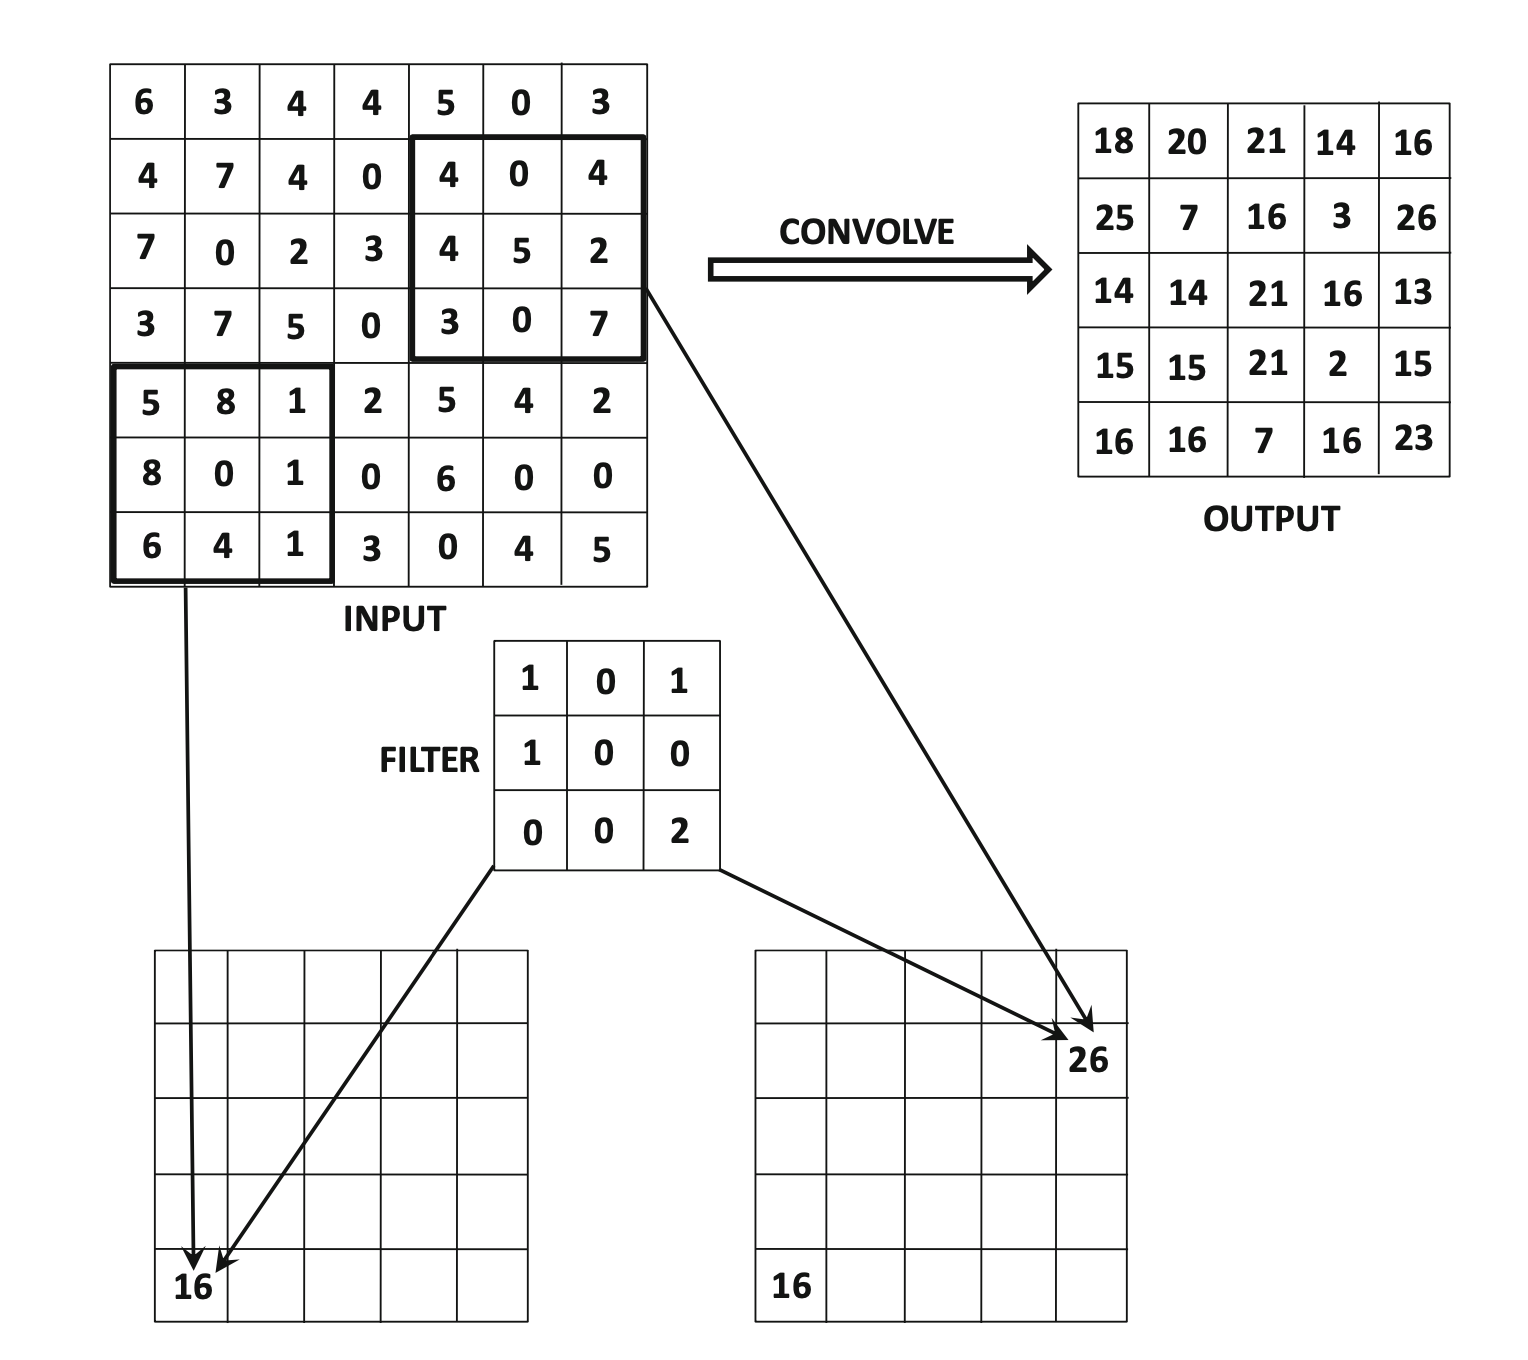
\includegraphics[width=10cm]{kapitel2/conv_layers.png}
        \caption[Die Faltung in einem CNN]{Die Faltungsoperation geschieht durch eine Punktprodukt Operation des Filters, was über alle räumlichen Positionen wiederholt wird aus \cite*[321]{Aggarwal2018}.}
        \label{Kap2:Conv}
    \end{figure}

    \subsection{Padding}
    Die Faltungsoperation verringert die Größe der $(q + 1)$-ten Schicht im Vergleich zur Größe der $q$-ten Schicht. Diese Art der Größenreduzierung ist im Allgemeinen nicht wünschenswert, da sie dazu neigt, einige Informationen entlang der Bildränder zu verlieren. Dieses Problem kann durch \textbf{Auffüllen} (padding) gelöst werden. Beim Auffüllen werden neue Werte rund um die Ränder der Feature-Map hinzugefügt. Der Wert jedes dieser aufgefüllten Feature-Werte wird auf 0 gesetzt, unabhängig davon, ob die Eingabe oder die ausgeblendeten Ebenen aufgefüllt werden. Diese Bereiche tragen nicht zum endgültigen Punktprodukt bei, da ihre Werte auf 0 gesetzt sind. Ein Teil des Filters aus den Rändern der Schicht wird \enquote{herausragt} und dann durch das Durchführen des Punktprodukts nur über den Teil der Ebene, in dem die Werte definiert sind ersetzt \cite*[323]{Aggarwal2018}.


\subsection{Pooling Layer}
Es ist üblich, regelmäßig eine \textbf{Pooling Ebene} zwischen aufeinanderfolgenden Faltungsebenen in eine ConvNet-Architektur einzufügen. Die Funktion dieser Ebenene besteht darin, die räumliche Größe der Darstellung schrittweise zu verringern, um die Anzahl der Parameter und die Berechnung im Netzwerk zu verringern und damit auch die Überanpassung zu steuern. Die Pooling-Ebene arbeitet unabhängig mit jedem Tiefenabschnitt der Eingabe und ändert die Größe räumlich mithilfe der MAX-Operation. Die gebräuchlichste Form ist eine Pooling-Ebene mit Filtern der Größe \textit{2x2}, die mit einem\textbf{ Schritt} (Stride) von 2 Downsamples pro Tiefenscheibe in der Eingabe um 2 entlang der Breite und Höhe angewendet werden, wobei 75\% der Aktivierungen verworfen werden. Jede MAX-Operation würde in diesem Fall maximal 4 Zahlen annehmen. Der \textit{Volumen} bleibt unverändert \cite*{StanfordUniversityCoursecs231n2018a}.

\begin{figure}[H]
    \centering
    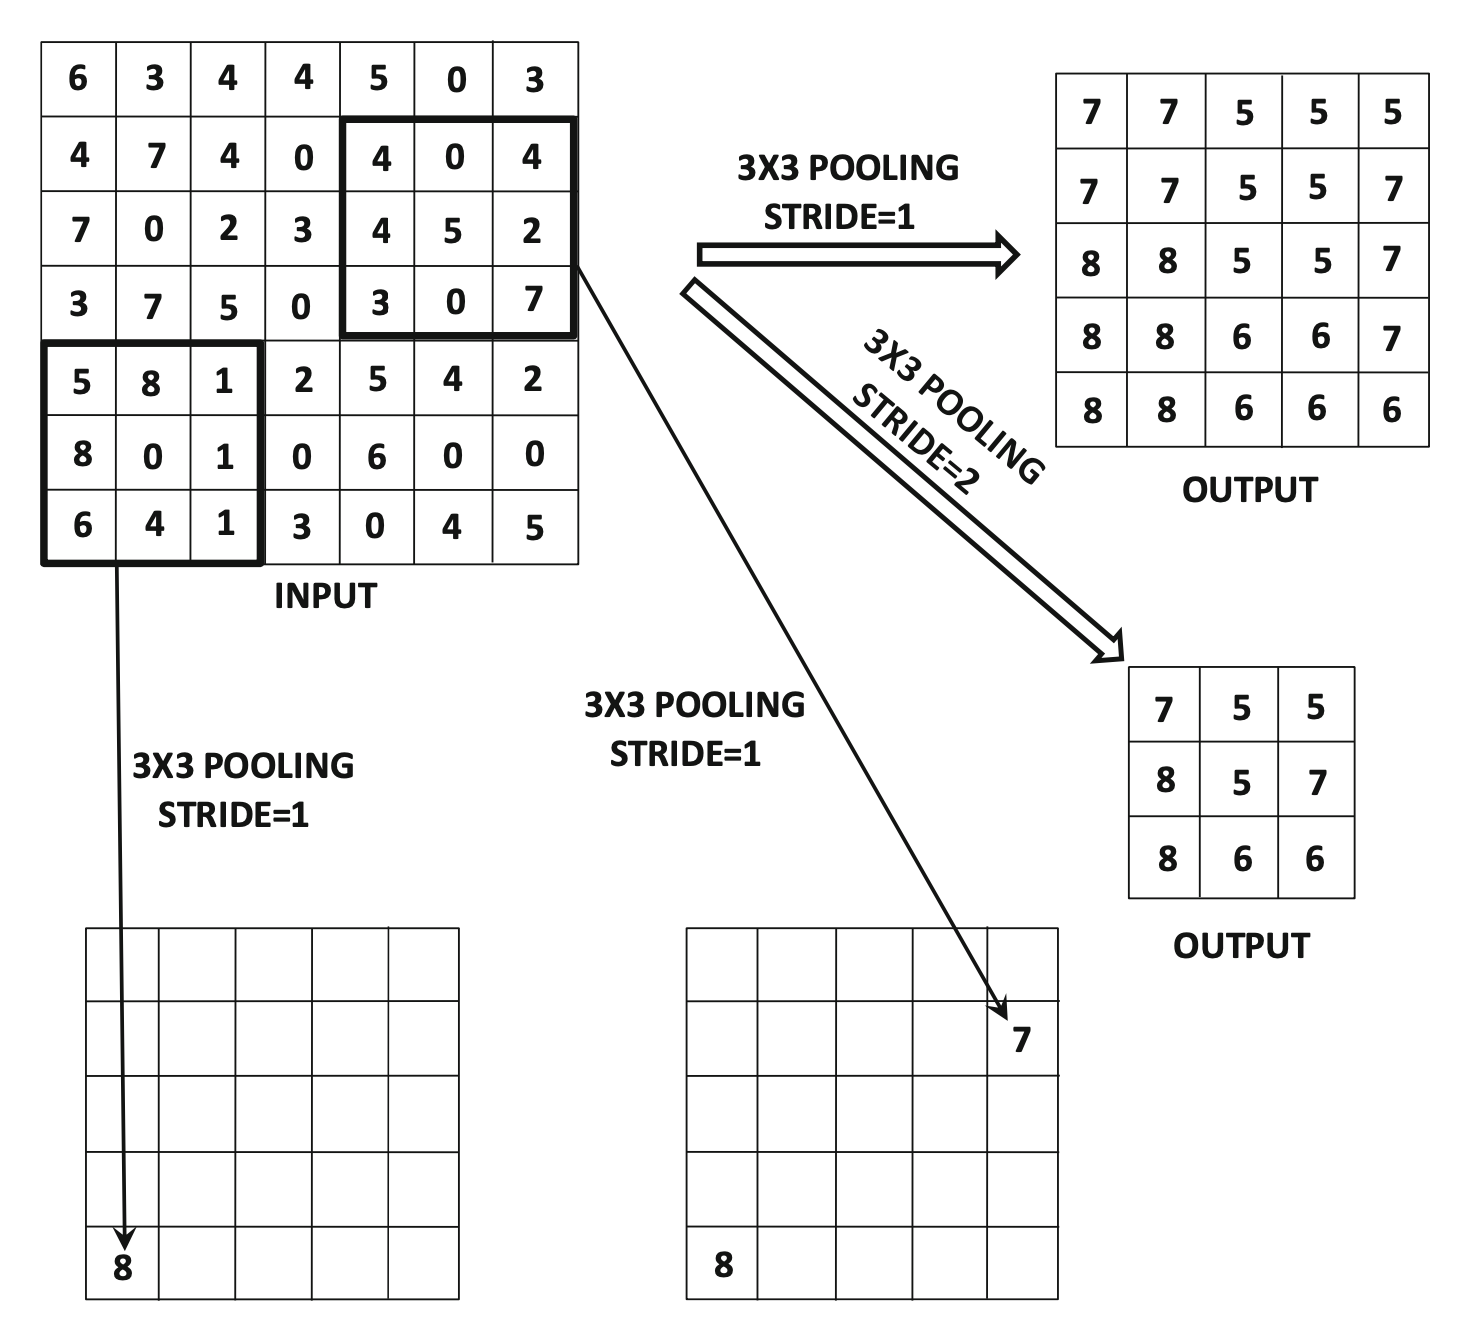
\includegraphics[width=9cm]{kapitel2/maxpooling.png}
    \caption[Max-Pooling]{Ein Beispiel für ein Max-Pooling einer Aktivierungskarte der Größe 7 × 7 mit Stride von 1 und 2. Ein Stride von 1 erzeugt eine 5 × 5-Aktivierungskarte mit stark wiederholten Elementen aufgrund der Maximierung in überlappenden Regionen. Ein Stride von 2 erzeugt eine 3 × 3-Aktivierungskarte mit weniger Überlappung \cite*[326]{Aggarwal2018}.}
    \label{Kap2:Pooling}
\end{figure}


\subsection{Vollständig verbundene Ebenen}
Am Ende wird die sogenannte \textbf{vollständig verbundene Ebenen} des Netzwerkes verwendet, um Klassenwerte zu berechnen, die als Ausgabe des Netzwerks dienen sollen. In einem traditionellen vorwärtsgerichteten Neuronalen Netzwerk wird jedes Eingangsneuron mit jedem Ausgangsneuron in der nächsten Schicht verbunden. Dies wird auch als vollständig verbundene Schicht bezeichnet. Der einzige Unterschied zwischen der vollständig verbundene Ebene und Faltungsschichten besteht darin, dass die Neuronen in der Faltungsschicht nur mit einer lokalen Region der Eingabe verbunden ist. Die Neuronen in beiden Schichten berechnen jedoch immer noch Punktprodukte, sodass ihre funktionale Form identisch ist. Zwischen beiden Schichten ist eine Konvertierung möglich \cite*{StanfordUniversityCoursecs231n2018a}.



\chapter{Die Natürliche Sprache}\label{ch3}


Die \textit{Verarbeitung natürlicher Sprache} (\enquote{NLP}) ist ein theoretisch motivierter Bereich von Computertechniken, zum Analysieren und Darstellen natürlich vorkommender Texte auf einer oder mehreren Ebenen der Sprachanalyse, um eine menschenähnliche Sprachverarbeitung für eine Reihe von Aufgaben oder Anwendungen zu erreichen \cite*{Liddy}.

Der Umgang mit Textdaten ist problematisch, da heutige Computer, Skripte und Modelle für maschinelles Lernen, keinen Text im menschlichen Sinne lesen und verstehen können. Wörter können viele verschiedene Assoziationen aufrufen. Diese sprachlichen Assoziationen sind das Ergebnis recht komplexer Berechnungen beim Menschen. ML-Modelle haben dieses vorgefertigte Verständnis der Bedeutung nicht.


\section{Tokenisierung durch Reguläre Ausdrücke}
Die Segmentierung eines Textes in seine Einheiten ist die erste Voraussetzung für dessen Weiterverarbeitung. In der Informatik können einzelne Wörter bzw. \enquote{Tokens} z.B. durch Leerzeichen voneinander abgetrennt werden. \textit{Reguläre Ausdrücke} können die Tokenisierung verbessern. Reguläre Ausdrücke können dabei helfen die Sprache so zu trennen, wie angegeben. Sie ist eine Sprache. Diese Sprache wird in allen Computersprachen verwendet. Formal ist ein regulärer Ausdruck eine algebraische Notation zur Charakterisierung einer Reihe von Zeichenfolgen. Sie sind besonders nützlich für die Suche in Texten, wenn ein Muster gesucht wird und ein Korpus von Texten durchsucht werden muss. Eine Suchfunktion für reguläre Ausdrücke durchsucht den Korpus und gibt alle Texte zurück, die dem Muster entsprechen. Der Korpus kann ein einzelnes Dokument oder eine Sammlung sein \cite*[3]{Jurafskya}. Reguläre Ausdrücke sind also bestimmte Regeln die Muster in einem Text erkennen lassen. Neben der Tokenisierung können sie auch für das extrahieren von Informationen aus Textsequenzen verwendet werden.

\section{N-Gramm}

Sprachmodelle sind Wortfolgen, zu denen Wahrscheinlichkeiten zugewiesen wurden. Das einfachste Sprachmodell ist das \textit{N-Gramm} Sprachmodell. Es ist eine Folge von N Wörtern (ein 2-Gramm oder Bigramm ist eine Folge von zwei Wörtern usw.). N-Gramm wird meistens dafür verwendet, um das nächste Wort in aus einer Sequenz vorherzusagen \cite*[31]{Jurafskya}. Angenommen ein Korpus besteht aus folgenden 4 Sätzen:

\begin{enumerate}
    \item Es regnet in Berlin.
    \item Es regnet in Köln und es ist 10 Grad.
    \item Es regnet und hagelt in ganz Deutschland.
    \item In Deutschland herrscht Regen.
\end{enumerate}

Um die Wahrscheinlichkeit \textit{P (regnet | in)} herauszufinden, wird die Anzahl des Wortes \enquote{regnet} im Korpus gezählt. Es wird gezählt, wie oft \enquote{regnet} und \enquote{in} zusammen vorkommen (2 Mal) und dieses wird dividiert durch 3, da \enquote{regnet} insgesamt 3 Mal im Korpus vorkommt. Das Bigramm \enquote{regnet in} hat also eine Wahrscheinlichkeit von 2/3.

\section{Part-of-Speech Tagging}
\textit{Part-of-Speech Tagging} ist der Prozess des Zuweisens eines Tags zu jedem Wortm auseinem Eingabetext. Die Eingabe ist eine Folge von tokenisierten Wörtern und einem \enquote{Tagset}, und die Ausgabe ist eine Folge von Tags, eines pro Token \cite*[148]{Jurafskya}. Je nach Sprache gibt es verschiedene \enquote{Tagger}, für das Deutsche gibt es das Stuttgart-Tübingen-Tagset\cite*{tagger}, einige Tags können aus der Tabelle~\ref{STTS} entnommen werden. Die Tagger wurden ursprünglich manuell erfasst und in heutiger Zeit durch das Maschinelle Lernen automatisiert.



\begin{table}[h]
    \caption{Beispiele aus dem Stuttgart-Tübingen-Tagset}
    \label{STTS}
    \renewcommand{\arraystretch}{1.2}
    \centering
    \sffamily
    \begin{footnotesize}
        \begin{tabular}{l l l}
            \toprule
            \textbf{POS} & \textbf{Beschreibung}                  & \textbf{Beispiel}                                  \\
            \midrule
            ADJA         & attributives Adjektiv                  & das \textit{große} Haus                            \\
            ADJD         & adverbiales oder prädikatives Adjektiv & er fährt \textit{schnell}, er ist \textit{schnell} \\
            ADV          & Adverb                                 & \textit{schon}, \textit{bald}, doch                \\
            NE           & Eigennamen                             & \textit{Hans}, \textit{Hamburg}, \textit{HSV}      \\
            NN           & normales Nomen                         & \textit{Tisch}, \textit{Herr}, das \textit{Reisen} \\
            VVFIN        & finites Verb, voll                     & du \textit{gehst}, wir \textit{kommen} an          \\
            \bottomrule
        \end{tabular}
    \end{footnotesize}
    \rmfamily
\end{table}




\section{One-Hot-Encoding}


Die verborgenen Schichten eines mehrschichtigen neuronalen Netzwerks lernen die Eingaben des Netzwerks so darzustellen, dass die Ausgaben leicht vorhergesagt werden können. Dies wird demonstriert, indem ein mehrschichtiges neuronales Netzwerk trainiert wird, um das nächste Wort in einer Sequenz aus einem lokalen Kontext vorheriger Wörter vorherzusagen \cite*{Bengio2003}. Jedes Wort im Kontext wird dem Netzwerk als \enquote{Eins-aus-N-Vektor} dargestellt, d.h. eine Komponente hat den Wert 1 und der Rest ist 0, dieses Verfahren wird auch als \textit{One-Hot-Encoding} bezeichnet. In einem \textit{Sprachmodell} lernen die anderen Schichten des Netzwerks, die Eingangsvektoren in einen Ausgangsvektor für das vorhergesagte nächste Wort umzuwandeln, umm die Wahrscheinlichkeit vorherzusagen, dass ein Wort im Vokabular als nächstes erscheinen wird \cite*{Lecun2015}. Das Netzwerk lernt \enquote{Wortvektoren}, die viele aktive Komponenten enthalten, von denen jede als separates Merkmal des Wortes interpretiert werden kann. Dieses Vorgehen wurde erstmals im Zusammenhang mit dem Lernen verteilter Darstellungen für Symbole demonstriert \cite*{Rumelhart1986}. Die semantischen Merkmale waren in der Eingabe nicht explizit vorhanden. Das Lernverfahren wurde als eine gute Möglichkeit entdeckt, die strukturierten Beziehungen zwischen den Eingabe- und Ausgabesymbolen in mehrere \enquote{Mikroregeln} zu zerlegen. Das Lernen von Wortvektoren hat sich auch als sehr gut erwiesen, wenn die Wortsequenzen aus einem großen Korpus stammen und die einzelnen Mikroregeln unzuverlässig sind \cite*{Bengio2003}.


Das One-Hot-Encoding ist also ein \enquote{spärlicher Vektor} in dem ein Element auf 1 gesetzt wird und alle anderen Elemente auf 0 gesetzt werden. One-Hot-Codierung wird üblicherweise verwendet, um Zeichenfolgen mit einer endlichen Menge möglicher Werte darzustellen. 



\begin{figure}[H]
    \centering
    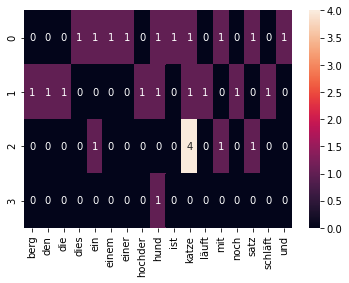
\includegraphics[width=8cm]{kapitel3/onhot.png}
    \caption[One-Hot-Encoding als Eingabematrix]{Die Grafik zeigt wie ein Beispielkorpus welches aus 5 Sätzen besteht, in einer Matrix dargestellt werden kann. Je nach Häufigkeit wird jedes Wort aus dem Wortschatz, entsprechend den Sätzen im Korpus abgebildet. Der Korpus besteht aus folgenden 5 Sätzen: \enquote{Dies ist ein Satz mit einer Katze und einem Hund.}, \enquote{Die Katze läuft den Berg hoch.}, \enquote{Der Hund schläft noch.}, \enquote{Ein Satz mit Katze Katze Katze Katze.} und \enquote{Ein Hund.}. Eigene Darstellung.}
    \label{OneHotGrafik}
\end{figure}





\section{Worteinbettungen}

Die numerischen Werte sollten so viel wie möglich von der sprachlichen Bedeutung eines Wortes erfassen. Eine gut ausgewählte, informative Eingabedarstellung kann einen massiven Einfluss auf die Gesamtleistung des Modells haben. \textit{Worteinbettungen} sind der vorherrschende Ansatz um dieses Problem zu lösen und so weit verbreitet, dass ihre Verwendung praktisch in jedem NLP-Projekt angenommen wird. Unabhängig davon, ob es ein Projekt in den Bereichen Textklassifikation, Sentimentanalyse oder maschinelle Übersetzung ist \cite*{Lecun2015}. Vektoren zur Darstellung von Wörtern werden im Allgemeinen als Einbettungen bezeichnet, da das Wort in einen bestimmten Vektorraum eingebettet wird \cite*[99]{Jurafskya}. 

%% fluch der dimensionalität
Eine Einbettung eine Übersetzung eines hochdimensionalen Vektors in einen niedrigdimensionalen Raum. Beispielsweise kann ein Satz als \enquote{spärlicher Vektor} mit Millionen Elementen (hochdimensional) dargestellt werden. Jede Zelle im Vektor repräsentiert ein separates Wort. Der Wert in einer Zelle gibt an, wie oft dieses Wort in einem Satz vorkommt. Da ein ein einzelner Satz wahrscheinlich nicht mehr als 50 Wörter hat, enthält fast jede Zelle eine 0. Die wenigen Zellen, die nicht 0 sind, enthalten eine kleine Zahl, welches die Häufigkeit des Auftretens dieses Wortes darstellt. Als \enquote{dichter Vektor} mit mehreren hundert Elementen (niedrigdimensional), wird ein gegebener Satz dargestellt, indem jedes Element ein Gleitkommawert zwischen 0 und 1 erhält. Dies ist die Einbettung. Die Werte können trainiert werden und sagen mehr aus als die \enquote{spärlichen Vektoren}.

\begin{figure}[H]
    \centering
    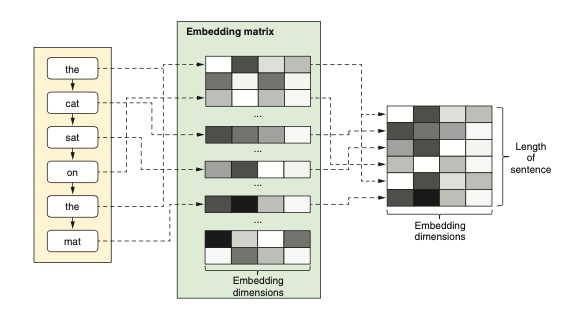
\includegraphics[width=13cm]{kapitel3/embd.png}
    \caption[Darstellung der Worteinbettungen]{Jede Zeile der Einbettungsmatrix entspricht einem Wort im Vokabular, und jede Spalte ist eine Einbettungsdimension. Die Werte der Elemente der Einbettungsmatrix, die im Diagramm als Graustufen dargestellt sind, werden zufällig ausgewählt und trainiert. Entnommen aus \cite[311]{cai2020deep}}
    \label{wordembgrau}
\end{figure}

\begin{table}[h]
    \caption{Vergleich des One-Hot-Encodings mit Worteinbettungen  \cite[312]{cai2020deep}}
    \label{componeembd}
    \renewcommand{\arraystretch}{1.2}
    \centering
    \sffamily
    \begin{footnotesize}
        \begin{tabular}{l l l }
            \toprule
                           & \textbf{One-Hot-Encoding} & \textbf{Worteinbettungen} & \textbf{}\\
        
            \textbf{Hartkodiert} & ja & nein, gelernt: Die Einbettungsmatrix ist ein                  \\
            & & trainierbarer Gewichtsparameter. Die Werte   \\
            & & spiegeln die semantische Struktur    \\
            & & des Wortschatzes nach dem Training wider. \\
            \\
            \textbf{Dichte}  & spärlich, die meisten Elemente                  & dicht, Elemente nehmen ständig              \\
            & sind Null, einige Eins. & wechselnde Werte an \\ 
            \\
            \textbf{Skalierbarkeit}  & nicht skalierbar,                 & skalierbar. Die Einbettungsgröße             \\
            & Die Größe des Vektors ist proportional  & muss nicht mit der Anzahl \\ 
            & zur Größe des Vokabulars. &  der Wörter im Vokabular zunehmen. \\
            \\
            \bottomrule
        \end{tabular}
    \end{footnotesize}
    \rmfamily
\end{table}




\section{Word2Vec}
\textit{Word2Vec} \cite*{Mikolov2013} Worteinbettungen sind Vektordarstellungen von Wörtern, die normalerweise von einem Modell gelernt werden, wenn große Textmengen als Eingabe eingegeben werden (z. B. Texte aus Wikipedia, Wissenschaft, Nachrichten, Artikel usw.). Diese Darstellung von Wörtern erfasst die semantische Ähnlichkeit zwischen Wörtern unter anderen Eigenschaften. Word2Vec-Worteinbettungen werden so gelernt, dass der Abstand zwischen Vektoren für Wörter mit enger Bedeutung (z. B. \enquote{König} und \enquote{Königin}) näher ist als der Abstand für Wörter mit völlig unterschiedlichen Bedeutungen (z. B. \enquote{König} und \enquote{Katze}).

Bei der One-Hot-Codierung sind die Wörter \enquote{gut} und \enquote{großartig} genauso unterschiedlich wie \enquote{Tag} und \enquote{Nacht}. Hier kommt die Idee, verteilte Darstellungen zu erzeugen. Intuitiv wird eine gewisse Abhängigkeit eines Wortes von den anderen Wörtern eingeführt. Die Wörter im Kontext dieses Wortes würden einen größeren Anteil dieser Abhängigkeit erhalten. In der One-Hot Darstellung dagegen, sind alle Wörter unabhängig voneinander.

\begin{figure}[H]
    \centering
    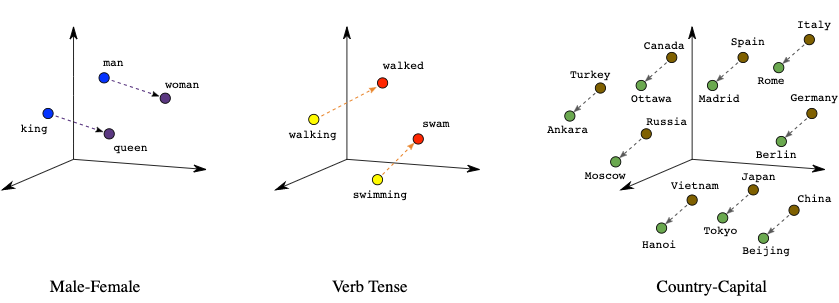
\includegraphics[width=14cm]{kapitel3/wordem.png}
    \caption[Worteinbettungen erzeugen Analogien zwischen Wörtern]{Durch Worteinbettungen können interessante Analogien zwischen einzelnen Wörtern gefunden werden. (Entnommen aus \cite*{wordemdgood})}
    \label{Word2Vec1}
\end{figure}



\section{Word2Vec mit der Skip-Gram Architektur}

Wörter können als spärliche, lange Vektoren mit vielen Dimensionen dargestellt werden. Eine alternative Methode ist die Darstellung eines Wortes mit der Verwendung von kurzen Vektoren, mit einer Länge von 50-1000 und einer großen dichte (die meisten Werte sind nicht Null). Es stellt sich heraus, dass dichte Vektoren in NLP-Aufgaben bessere Ergebnisse abgeben, als spärliche Vektoren. Wenn beispielsweise 100-dimensionale Worteinbettungen als Merkmal verwendet wird, kann ein Klassifikator nur 100 Gewichte lernen, um die Bedeutung des Wortes darzustellen. Wenn  stattdessen einen 50.000-dimensionalen Vektor eingeben wird, müsste ein Klassifikator Zehntausende von Gewichten für jede der spärlichen Dimensionen lernen. Dichte Vektoren können besser verallgemeinern und helfen eine Überanpassung zu vermeiden, da sie weniger Parameter als spärliche Vektoren mit expliziten Zählungen enthalten. Schließlich können dichte Vektoren die Synonyme besser erfassen als spärliche Vektoren. Zum Beispiel sind \enquote{Auto} und \enquote{Automobil} Synonyme und können beide im gleichen Zusammenhang verwendet werden. In einer typischen spärlichen Vektordarstellung sind beide Dimensionen unterschiedliche Dimensionen. Da die Beziehung zwischen diesen beiden Dimensionen nicht modelliert wird, können spärliche Vektoren möglicherweise die Ähnlichkeit zwischen Auto und Automobil als Nachbarn nicht erfassen \cite*[110-111]{Jurafskya}.


\begin{figure}[H]
    \centering
    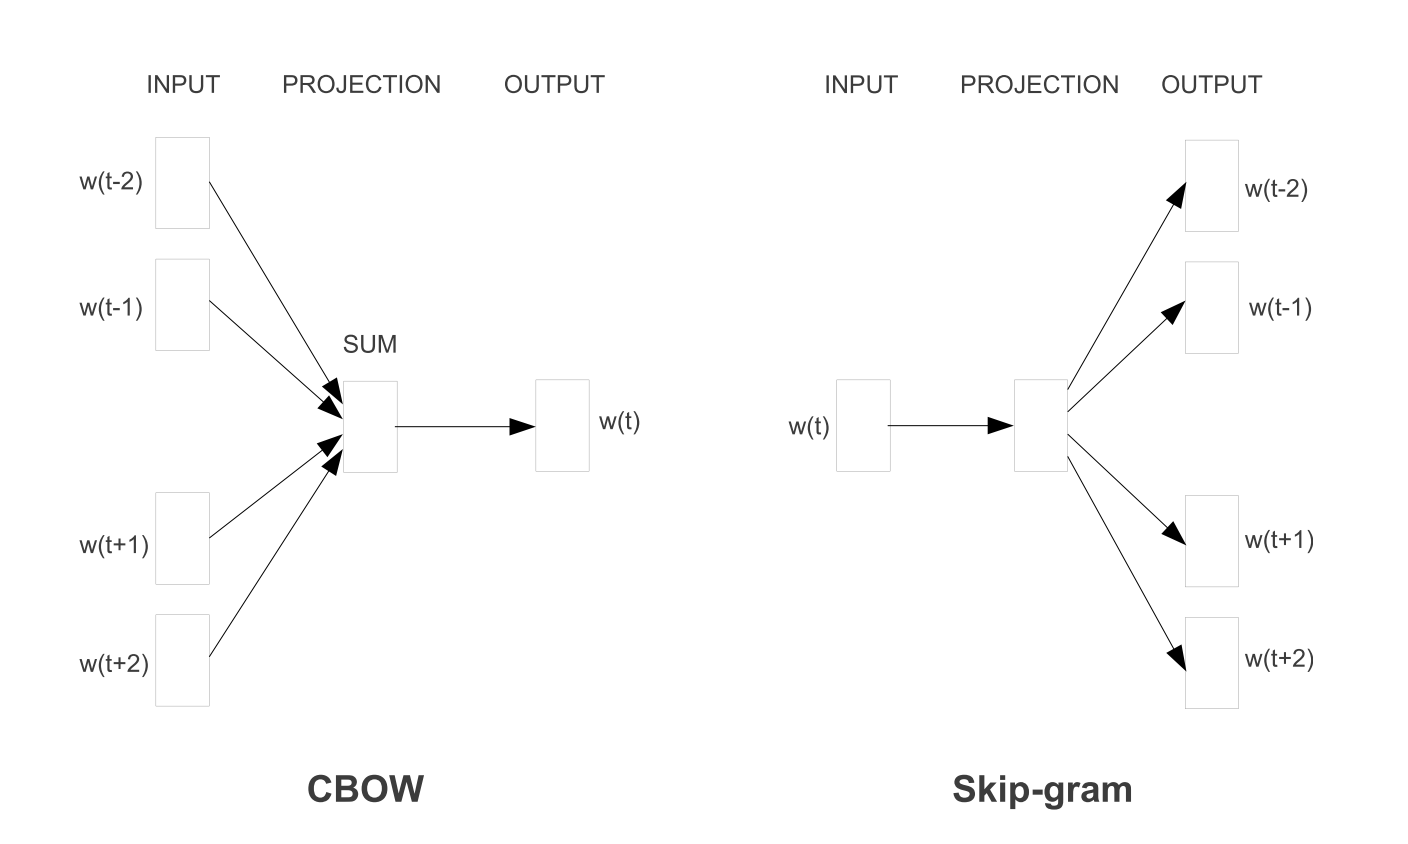
\includegraphics[width=12cm]{kapitel3/cbowskipgr.png}
    \caption[Vergleich zwischen CBOW und Skip-Gram Architektur]{Die CBOW-Architektur sagt das aktuelle Wort basierend auf dem Kontext voraus, während das Skip-Gramm die umgebenden Wörter voraussagt, wenn das aktuelle Wort gegeben ist aus \cite*{Mikolov}).}
    \label{cbowskipgr}
\end{figure}

Der Skip-Gram-Algorithmus ist einer von zwei Algorithmen in einem Softwarepaket namens \textit{Word2Vec} \cite*{Mikolov2013}\cite*{Mikolov}. Die Intuition von Word2Vec ist, dass anstatt zu zählen, wie of jedes Wort $w$ in der Nähe von einem anderen Wort vorkommt, einen Klassifikator für eine binäre Vorhersageaufgabe zu trainieren. Die erlernten Gewichte werden dann als Worteinbettungen bezeichnet \cite*[111]{Jurafskya}. Dabei wird ein Zielwort $t$ mit Kandidaten aus dem Kontext \textit{c} in ein \textit{Tupel} gesetzt. \textit{P(+|t,c)} sagt dann aus, wie wahrscheinlich es ist, dass ein Kontextwort \textit{c} ein echter Kontext ist. Zum Beispiel sei gegeben der Satz \enquote{Wir essen Spaghetti zum Abendessen...}. Wenn der Kontext von $\pm 2$ Wörter betrachtet wird, und \textit{t} das Zielwort \enquote{essen} ist, wird die Klassifikation für das Tupel \textit{(essen,spaghetti)} \enquote{true} und für das Tupel \textit{(essen,auto)} \enquote{false} zurückgeben \cite*[111]{Jurafskya}.


Die Ähnlichkeit eines Wortes zu einem anderen Wort, kann durch den Skalarprodukt berechnet werden. Dies ist zunächst nur eine Zahl zwischen $-\infty$ und $+\infty$. Um daraus eine Wahrscheinlichkeit zu berechnen, wird die \textit{sigmoid}-Funktion $\sigma(x)$ angewendet. Die Logistikfunktion gibt eine Zahl zwischen 0 und 1 zurück. Um die Wahrscheinlichkeit zu berechnen, muss gewährleistet werden, dass die Summe \textit{c ist das Kontextwort} und \textit{c ist nicht das Kontextwort} eine 1 ergeben \cite*[112]{Jurafskya}.

\begin{equation} \label{Formel3_2}
    P(-|t,c) = 1-P(+|t,c) = \frac{e^{-t\cdot c}}{1+e^{-t\cdot c}}
\end{equation}
\myequations{Wahrscheinlichkeiten bei Skip-Gram}

Skip-Gramm macht die starke, aber sehr nützliche vereinfachende Annahme, dass alle Kontextwörter unabhängig sind, so dass ihre Wahrscheinlichkeiten multipliziert werden können \cite*[112]{Jurafskya}:

\begin{equation} \label{Formel3_3}
    P(+|t,c_{1:k}) = \prod ^{k}_{i=1}\frac{1}{1+e^{-t\cdot c_{i}}}
\end{equation}
\myequations{Multiplikationen der Skip-Gram}


Word2Vec lernt Einbettungen, indem es mit einem anfänglichen Satz von Einbettungsvektoren beginnt und dann die Einbettung jedes Wortes $w$ iterativ verschiebt, um mehr in der Nähe der Einbettungen von Wörtern zu kommen, die ähneln. Für das Training eines binären Klasifikators sind zunächst negative Beispiele nötig. Das Skip-Gram benötigt mehr negative als positive Beispiele für das Training. Das Verhältnis zwischen positiven und negativen Beispielen wird mit einem Parameter $k$ festgelegt. Für jede Trainingseinheit \textit{t, c} werden \textit{k} negative Stichproben erstellt, die jeweils aus dem Ziel \textit{t} und einem \enquote{noise word} besteht. Ein \enquote{noise word} is ein zufälliges Wort aus dem Lexikon, das nicht das Zielwort \textit{t} sein darf \cite*[113]{Jurafskya}.

Das Ziel des Lernalgorithmus besteht darin, mittels gegebenen positiven und negativen Beispielen diese Einbettungen so anzupassen, dass die Ähnlichkeit der Ziel- und Kontextwortpaare \textit{(t, c)} aus den positiven Beispielen maximiert werden und die Ähnlichkeit der Paare \textit{(t, c)} aus den negativen Beispielen minimiert wird. Formell lässt sich dieses mit folgender Formel ausdrücken:

\begin{gather} \label{Formel3_5}
    L(\theta) = \sum_{(t,c)\in +}\log P(+|t,c)+\sum_{(t,c)\in -} \log P(-|t,c) =  \notag\\
    \log \sigma(c \cdot t)+\sum^{k}_{i=1}\log \sigma(-n_{i} \cdot t) = \notag\\
    \log \frac{1}{1+e^{-c \cdot t}}+\sum^{k}_{i=1}\log\frac{1}{1+e^{n_{1} \cdot t}}.
\end{gather}
\myequations{Der Lernalgorithmus des Skip-Gram}

Die stochastische Gradientenabstieg kann verwendet werden, um dieses Ziel zu erreichen, indem die Parameter (die Einbettungen für jedes Zielwort $t$ und jedes Kontextwort oder \enquote{noise word} $c$ im Vokabular) iterativ modifiziert werden \cite*[114]{Jurafskya}.


\section{CNN in der Textverarbeitung}
Anstelle von Bildpixeln sind die Eingaben für die meisten NLP-Aufgaben Sätze oder Dokumente, die als eine Matrix dargestellt werden können. Jede Zeile der Matrix entspricht einem Token, normalerweise einem Wort, aber es kann sich auch um ein Zeichen handeln. Das heißt, jede Zeile ist ein Vektor, welches aus Wörtern und Zeichen besteht. Typischerweise sind diese Vektoren Worteinbettungen (niedrigdimensionale Darstellungen) wie Word2Vec oder GloVe, aber sie können auch One-Hot-Vektoren sein, die das Wort in ein Vokabular indizieren \cite*{Zhang}.

In der Vision (z.B. Klassifikation von Bildern) \enquote{gleiten} die Filter über lokale \enquote{patches} eines Bildes, in NLP jedoch geleitet der Filter über die ganze Zeile der Matrix (Wörter). Daher entspricht die Breite der Filter normalerweise der Breite der Eingabematrix. Die Höhe kann variieren, aber \enquote{Schiebefenster} mit jeweils mehr als 2-5 Wörtern sind typisch. Pixel, die nahe beieinander liegen, sind wahrscheinlich verwandt (Teil desselben Objekts), aber das Gleiche gilt nicht immer für Wörter. In vielen Sprachen können Teile von Phrasen durch mehrere andere Wörter getrennt werden. Der kompositorische Aspekt ist ebenfalls nicht offensichtlich. Es ist klar, dass Wörter in gewisser Weise zusammengesetzt sind, wie ein Adjektiv, das ein Substantiv modifiziert, aber wie genau dies funktioniert, was Darstellungen auf höherer Ebene tatsächlich \enquote{bedeuten}, ist nicht so offensichtlich wie im Fall von Computer Vision. Angesichts all dessen, scheinen CNNs nicht gut für NLP-Aufgaben geeignet zu sein. Wiederkehrende neuronale Netze (RNNs) sind intuitiver. Sie ähneln der Art und Weise, wie Menschen die Sprache verarbeiten (oder zumindest wie Menschen denken, dass sie die Sprache verarbeiten). Menschen lesen nacheinander von links nach rechts. Es stellt sich aber heraus, dass CNNs, die auf NLP-Probleme angewendet werden, recht gut funktionieren. Ein großes Argument für CNNs ist, dass sie schnell sind. Faltungen sind ein zentraler Bestandteil der Computergrafik und werden auf der Hardwareebene auf GPUs implementiert. Mit einem großen Wortschatz kann das Berechnen schnell \enquote{teuer} werden. Faltungsfilter lernen automatisch gute Darstellungen, ohne das gesamte Vokabular darstellen zu müssen \cite*{widlml}.

\begin{figure}[H]
    \centering
    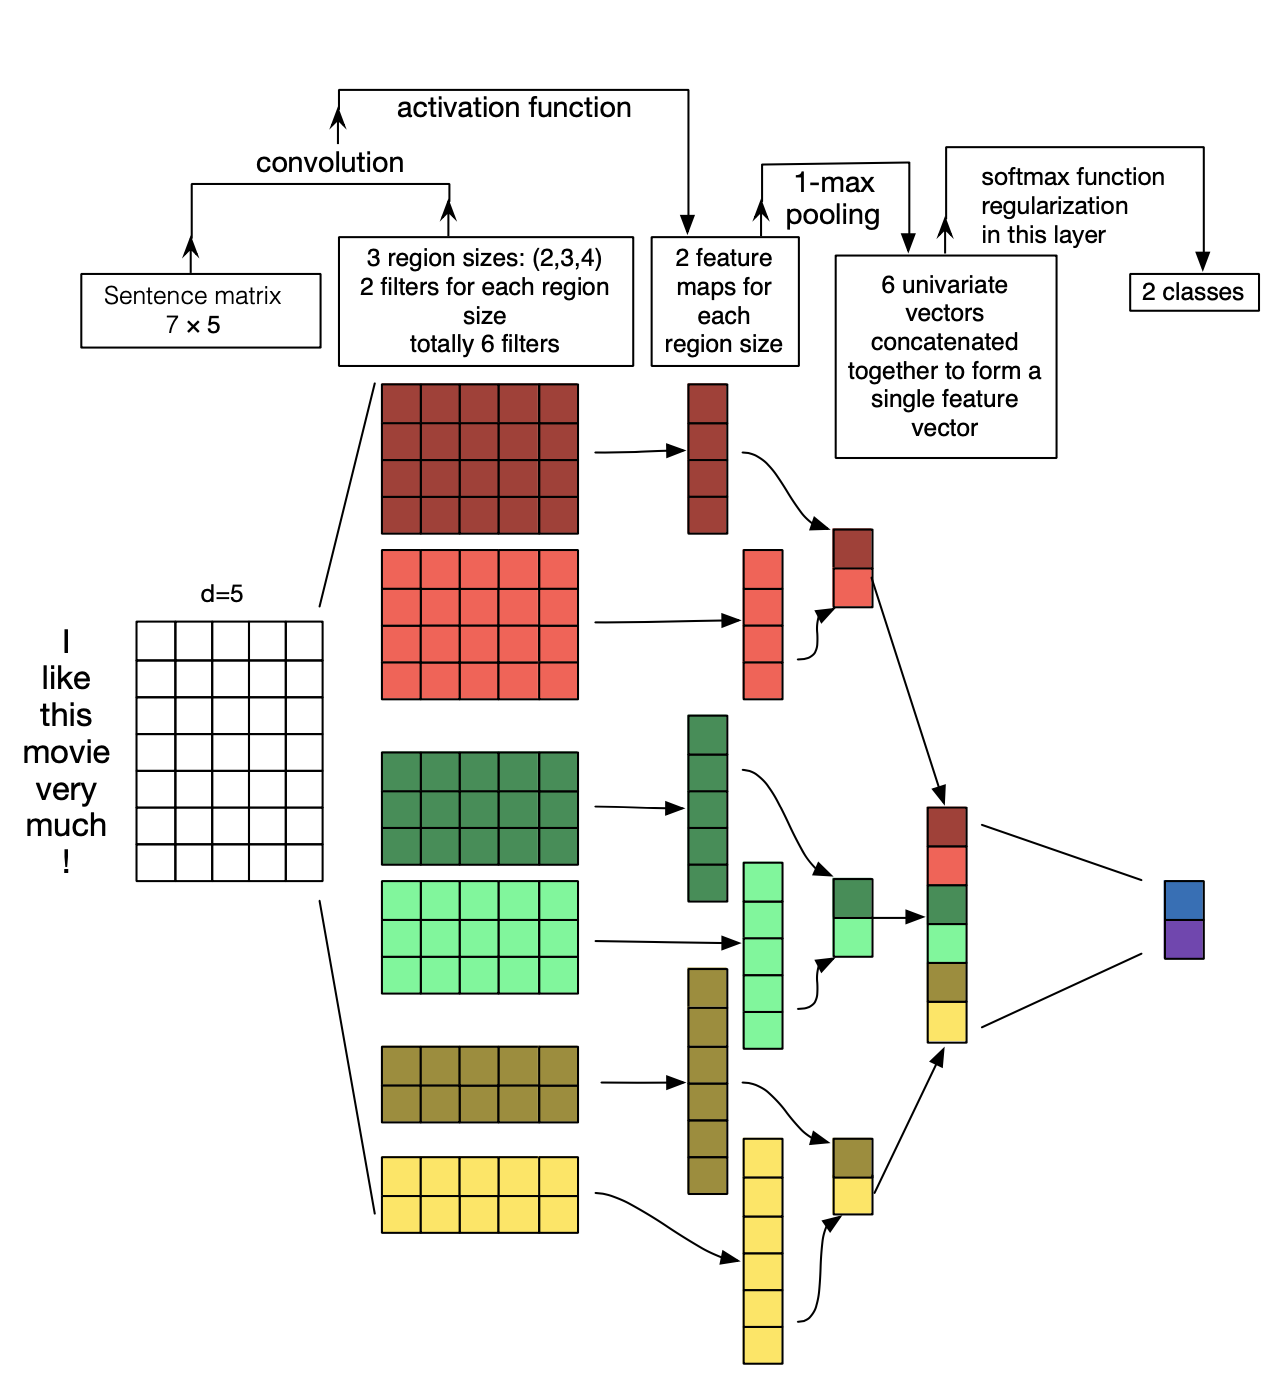
\includegraphics[width=9cm]{kapitel2/cnnnlp.png}
    \caption[CNN in der Textverarbeitung]{Illustration einer CNN-Architektur zur Satzklassifizierung. Es sind drei Filterbereichsgrößen vorhanden: 2, 3 und 4. Filter führen Faltungen in der Satzmatrix durch und generieren Feature-Maps (mit variabler Länge). Über jede Karte wird ein 1-Max-Pooling durchgeführt, d. H. die größte Anzahl von jeder Merkmalskarte wird aufgezeichnet. Somit wird aus allen sechs Karten ein univariater Merkmalsvektor erzeugt, und diese sechs Merkmale werden verkettet, um einen Merkmalsvektor für die vorletzte Schicht zu bilden. Die letzte softmax-Schicht empfängt dann diesen Merkmalsvektor als Eingabe und verwendet ihn zur Klassifizierung des Satzes an. Hier wird eine binäre Klassifikation angewendet und es gibt daher zwei mögliche Ausgangszustände \cite*{Zhang}.}
    \label{Kap2:Pooling}
\end{figure}

Eindimensionale CNNs können für Sequenzen wie Sätze verwendet werden. Der 1D-CNN-Algorithmus beinhaltet das Gleiten eines Kernels, wobei die Gleitbewegung in eine Richtung oder Dimension erfolgt. An jeder Gleitposition wird eine Schicht des Inputs extrahiert \cite[312-313]{cai2020deep}. Angenommen ein Satz besteht aus 9 Wörtern. Jedes Wort wird als Vektor dargestellt. Wenn ein Filter der Größe 2 vorhanden ist, gleitet dieser 8 Positionen nach unten, dieses ist die größe des \enquote{Kernels}. Im nächsten Schritt geschieht eine Punktprodukt Operation zwischen der Eingabe und dem Kernel. Dieses ist ein linearer Prozess und wird bis zum Ende wiederholt. 


\begin{figure}[H]
    \centering
    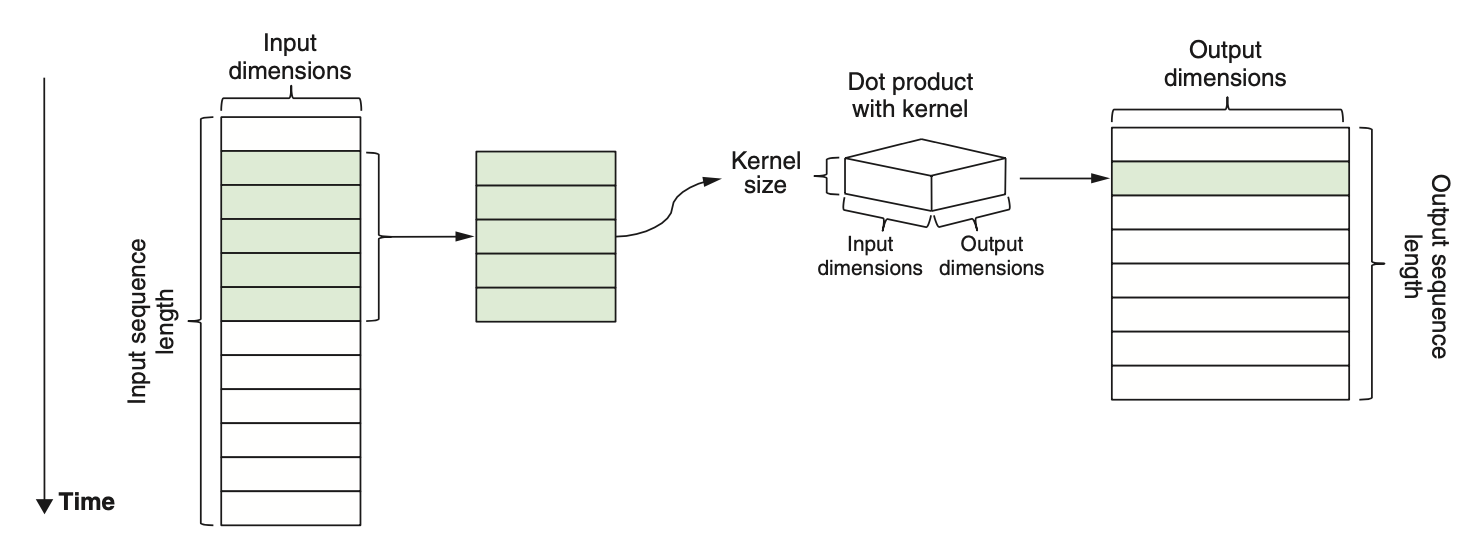
\includegraphics[width=13cm]{kapitel3/1dcn.png}
    \caption[1-dimensionale CNN]{Darstellung der Faltungsoperation beim 1D-CNN. Entnommen aus \cite[313]{cai2020deep}}
    \label{1dcnn}
\end{figure}

\chapter{Clickbaits und die Klassifizierung von Clickbaits}\label{ch4}


Clickbaits besitzen semantische und syntaktische Nuancen, auf die besonders vorgegangen werden muss. Dies geschieht in Form von analyse und vorverarbeitung der Titel. In diesem Abschnitt werden Ansätze aus der Literatur verglichen, die diese semantischen und syntaktischen Besonderheiten bearbeiten. In diesem Kapitel werden Ansätzte aus der Literatur vorgestellt, die die Aufgabe Clickbait Klassifizierung und die damit entstehenden Unteraufgaben wie das Sammeln von Daten, Einbetten der Wörter und schließlich entwickeln der Deep Learning Modelle haben.


\section{Was sind Clickbaits?}


Was sich hinter einer Schlagzeile, einem Titel verbirgt ist ohne weiteres nicht ersichtlich. Die meisten Menschen nehmen heutzutage Ihre Nachrichten über soziale Medien auf. Auf sozialen Medien werden meistens nur die Schlagzeilen gezeigt und wenn der Nutzer einen entsprechenden Eintrag interessant oder lesenswert findet, klickt er auf diesen Link. Das Wort Clickbait stammt aus den beiden Wörtern \enquote{Klick} und \enquote{Köder}, es ist also eine Falle. Viele Medienunternehmen, teilweise auch große, nutzen diese Falle um mehr Klicks zu generieren. Das Problem dabei ist es oftmals, dass die Nutzer durch die \enquote{Spannung} oder \enquote{Frage} in der Schlagzeile eine Erwartung haben, die nicht immer oder nur teilweise erfüllt wird. In der Studie von \cite*{Main} wurden ca. 1,6 Mio. Facebook-Posts untersucht und es wurde festgestellt, dass 25 bis 60\% der Fälle Clickbaits-Posts waren, je nach Medienunternehmen und Thema.

\begin{figure}[H]
    \centering
    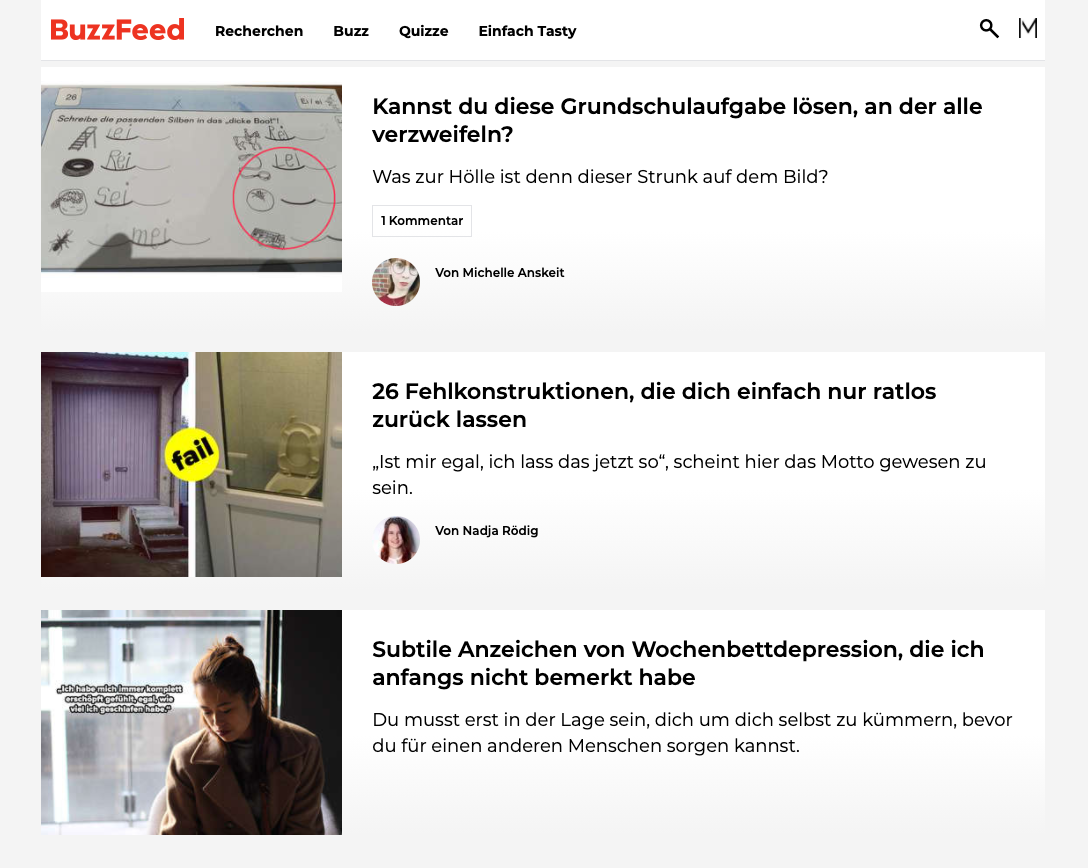
\includegraphics[width=11cm]{kapitel4/buzz.png}
    \caption[Beispiele von Clickbaits]{Beispiele von Clickbaits Nachrichten im Internet}
    \label{clckbPic}
\end{figure}

\begin{figure}[H]
    \centering
    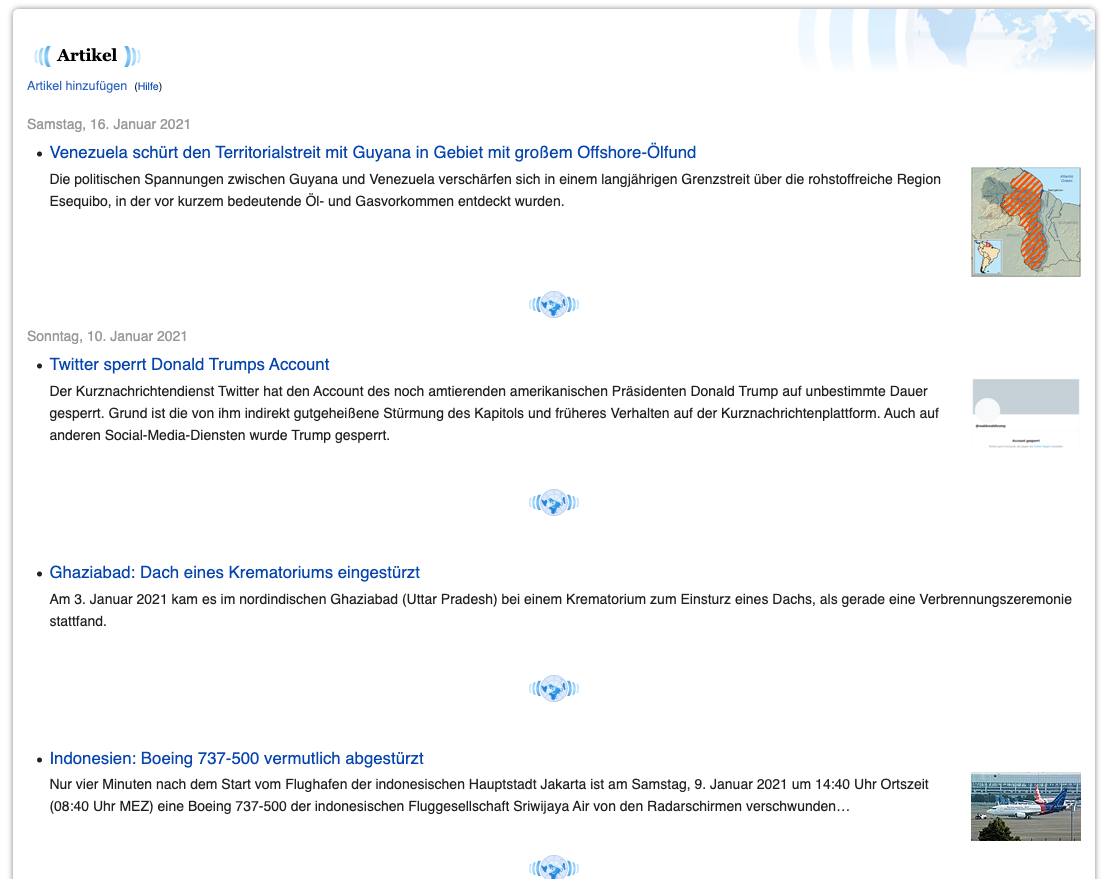
\includegraphics[width=11cm]{kapitel4/wikinews.png}
    \caption[Beispiele von Nicht-Clickbaits]{Beispiele von Nicht-Clickbaits Nachrichten im Internet}
    \label{clckbPic}
\end{figure}

Es gibt keine eindeutige Definition für Clickbaits. Clickbaits weisen unterschiedliche Formen. Nach \cite*{Biyani2016} sind Clickbaits, als eine Praxis um Klicks zu generieren, durch eine attraktive Überschrift, wessen Inhalt die Erwartungen nur teilweise oder gar nicht erfüllt. Clickbaits kann also eine Täuschung oder Trick der Medien betrachtet werden. Eine andere Definition \cite*{Potthasta} betrachtet das Thema Clickbait eher als Werbung für Onlineinhalte und die damit verbundene verbreitung oder viral gehen durch die sozialen Medien.

\begin{figure}[H]
    \centering
    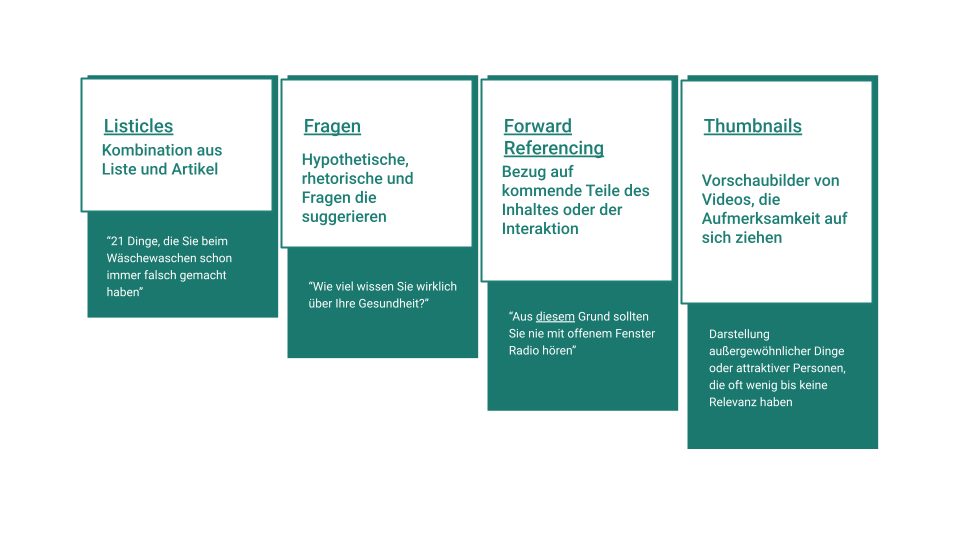
\includegraphics[width=15cm]{kapitel4/clickbaits.png}
    \caption[Die Kernformen des Clickbaits]{Die 4 Kernformen des Clickbaits in Anlehnung an \cite*[71]{Hrsg2020}}
    \label{TSNE}
\end{figure}

In \cite*[70-71]{Hrsg2020} werden CLickbaits formal in 4 Kategorien aufgeteilt. Der Autor bezieht sich dabei auf 4 Quellen und teilt Clickbaits als Listicles \cite*{Vijgen2014}, Fragen \cite*{Lai2014}, Forward Referencing \cite*{Blom2015} und Thumbnails \cite*{Zannettou2018} auf. Diese 4 Kategorien betrachtet der Autor als Kernkategorien. Aus \cite*[71]{Hrsg2020} werden Clickbaits außerdem in weitere Gestaltungsformen wie etwa, dass sie \enquote{Übertreibungen} sein können also falsche Versprechen geben, oder irreführend sind und unklar sein können.Es wird außerdem auf die unangemessene und vulgäre Sprache und der Formatierung, wie etwa den übertriebenen Gebrauch von Großschreibung oder Satzzeichen aufmerksam gemacht. Der Autor macht auf \cite*[75-76]{Hrsg2020} deutlich, dass Clickbaits kein neu eingesetztes Stilmittel im Journalismus sei. Schließlich verwendet der Autor den Begriff \enquote{Neugier} beim Leser. Leser wollen oftmals über Themen wie Tod, Gewalt, Sex und Prominente \cite*{Tenenboim2015} unterhalten werden.




\section{Wie werden Clickbaits klassifiziert?}
Mit der Arbeit aus \cite*{Chakrabortya} wurde eine Browser-Erweiterung erstellt, welches Clickbaits erkennen soll. Es wurden umfangreiche Daten sowohl für Clickbaits als auch für Nicht-Clickbait-Kategorien gesammelt. Für die Nicht-Clickbaits-Kategorien wurden 18.513 Wikinews Artikeln gesammelt. Der Vorteil dieser Artikel ist, dass diese von einer Community erstellt werden und jeder Nachrichtenartikel vor der Veröffentlichung von der Community geprüft werden. Es gibt Stilrichtlinien, die eingehalten werden müssen. Um Clickbaits zu finden, haben die Autoren manuell aus Seiten wie \enquote{Buzzfeed} oder \enquote{Upworthy} ca. 8000 Titel gecrawlt. Um falsche Negative zu vermeiden (d. h. die Artikel in diesen Bereichen, bei denen es sich nicht um Clickbaits handelt), wurden sechs Freiwillige rekrutiert um die Überschriften zu labeln. Schließlich wurden 7500 Titel zu jeder der beiden Kategorien zugefügt.

% \section{Analyse Textdaten}


Laut \cite*{Chakrabortya} sind die herkömmlichen Nicht-Clickbait Schlagzeilen kürzer als Clickbait Schlagzeilen. Traditionelle Schlagzeilen enthalten in der Regel meistens Wörter, die sich auf bestimmte Personen und Orte beziehen, während die Funktionswörter den Lesern zur Interpretation aus dem Kontext überlassen bleiben. Es wird hier als Beispiel gegeben \enquote{Visa-Deal oder kein Migranten-Deal, Türkei warnt EU}. Hier sind die meisten Wörter Inhaltswörter, die die wichtigsten Erkenntnisse aus der Geschichte zusammenfassen, und es gibt nur sehr wenige Verbindungsfunktionswörter zwischen den Inhaltswörtern. Auf der anderen Seite sind Clickbait Schlagzeilen länger. Die Sätze, enthalten sowohl Inhalts- als auch Funktionswörter. Ein Beispiel für solche Schlagzeilen ist \enquote{Ein 22-Jähriger, dessen Ehemann und Baby von einem betrunkenen Fahrer getötet wurden, hat ein Facebook-Plädoyer veröffentlicht}. Obwohl die Anzahl der Wörter in Clickbait-Schlagzeilen höher ist, ist die durchschnittliche Wortlänge kürzer. Es werden häufig Wörter verwendet wie \enquote{Sie werden}, \enquote{Sie sind}. Im Durchschnitt haben die Wörter bei den Clickbaits längere Abhängigkeiten als Nicht-Clickbaits. Der Hauptgrund ist die Existenz komplexerer Phrasensätze im Vergleich zu Schlagzeilen ohne Clickbait. Es ist außerdem zu sehen, dass in Clickbait-Schlagzeilen Stoppwörter häufiger verwendet werden. Clickbait Überschriften verwenden häufig Determinantien wie \enquote{ihre}, \enquote{meine}, die auf bestimmte Personen oder Dinge im Artikel verweisen. Die Verwendung Wörter dient in erster Linie dazu, den Benutzer neugierig auf das Objekt zu machen, auf das verwiesen wird, und ihn zu überzeugen, den Artikel weiter zu verfolgen. Um Daten zu erfassen, können auch Soziale Medien wie Twitter herangezogen werden, wie im Beispiel von \cite*{Potthast}.


% \section{Feature Selection}
Um lexikalischer und semantische und orthografische und morphologische Merkmale zu erfassen, benutzen die Autoren aus \cite*{Anand2019} Worteinbettungen und Zeicheneinbettungen, anstatt übermäßig Feature Selection auszuüben. Um Informationen außerhalb einzelner oder fester Wortfenster zu erfassen, untersuchten die Autoren dabei verschiedene RNN-Architekturen (Recurrent Neural Network) wie LSTM (Long Short Term Memory), GRU (Gated Recurrent Units) und Standard-RNNs. Dieses sind Wiederkehrende neuronale Netzwerkmodelle, die für sequentielle Daten wie Sprache und Text gut modelliert werden können.


Die Arbeit von \cite*{Agrawal2017} schlägt ein Modell vor, welches CNNs benutzt. CNNs werden für verschiedene Deep-Learning-Aufgaben verwendet. Es wurde nur eine Faltungsschicht in das CNN-Modell eingebaut. Die erste Schicht wird für das Einbetten der Wörter in Vektoren verwendet. Dabei wurden 2 verschiedene Worteinbettungen in Bezug genommen. Ein vortrainiertes und eines welches von Grund auf lernen musste und sich während des Trainings weiterentwickelt. In der nächsten Schicht werden Filter in verschiedenen Größen verwendet um Faltungen über Wortvektoren zu erzeugen.

Die Autoren der Arbeit aus \cite*{Pujahari} Clustern zunächst die aus den Schlagzeilen erstellten Vektoren mit der sogenannten t-SNE Methode nach \cite{VanDerMaaten2008}. Dieser Algorithmus \enquote{rekategorisiert} die Schlagzeilen in mehrere Gruppen und reduziert die vielen Dimensionen von Clickbaits im Datensatz. Die Autoren beginnen erst im nächsten Schritt mit dem Training. Dabei entstehen 11 Kategorien von Clickbaits (Mehrdeutig, Übertreibung oder Neckerei).


\begin{figure}[H]
    \centering
    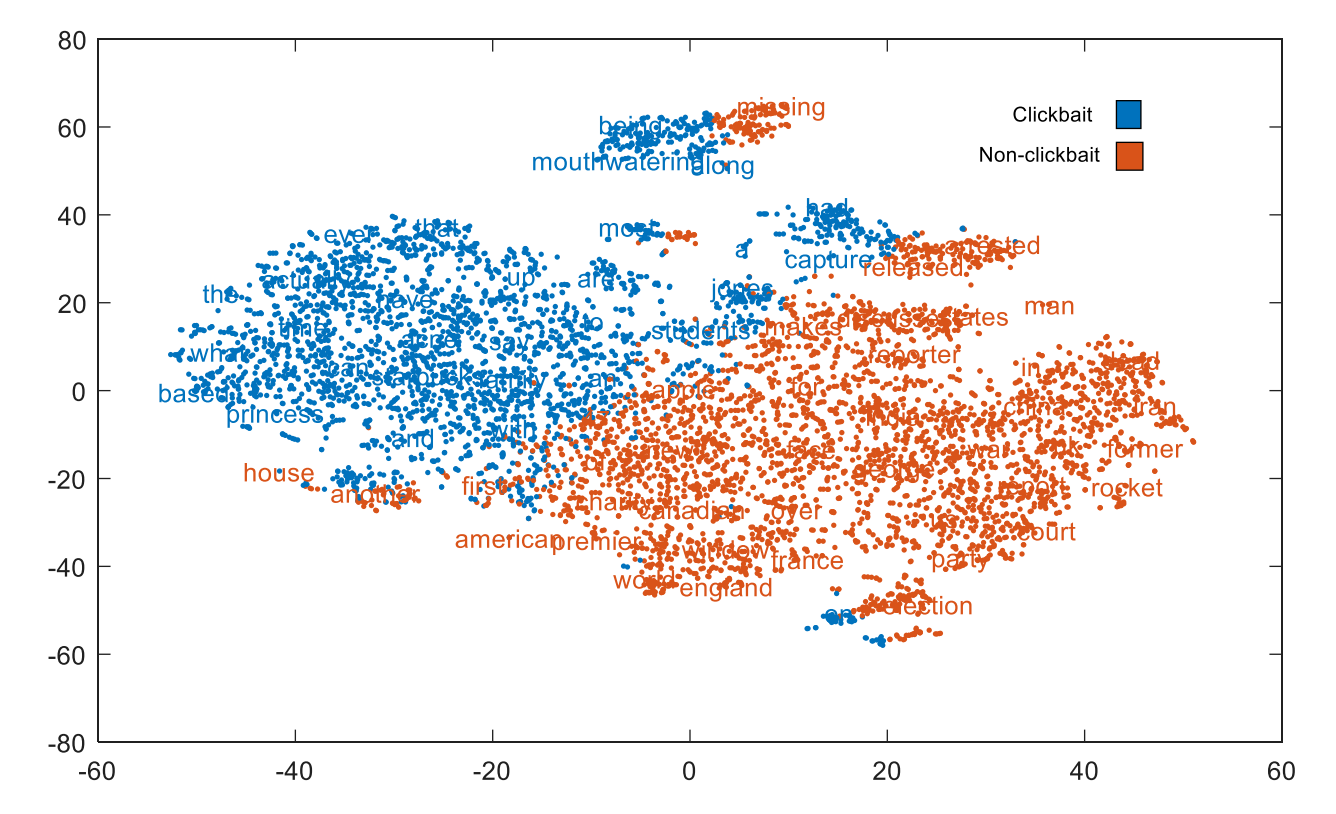
\includegraphics[width=12cm]{kapitel4/tsne.png}
    \caption[Clustering von Überschriften mit t-SNE]{Die Autoren verwenden das t-SNE Algorithmus nach \cite{VanDerMaaten2008} um die Dimensionen zu Reduzieren und es entstehen mehrere Unterkategorien von Clickbaits. Entnommen aus \cite*{Pujahari}.}
    \label{TSNE}
\end{figure}


\chapter{Implementierung}
\section{Konzeption und Methodik}


Das Konzept dieser Arbeit ist auf 3 Säulen aufgebaut. Erstens, das Sammeln, Speichern und Analyse der Daten und die Analyse der Daten, zweitens, das Entwickeln eines Deep Learning Modells, welches durch die gesammelten und angepassten Daten entsteht und drittens, das Implementieren und Einbetten des Modells in eine Benutzeroberfläsche, also in die Clientseite, siehe Abbildung~\ref{Kap5:Konzeption}.

\begin{figure}[H]
    \centering
    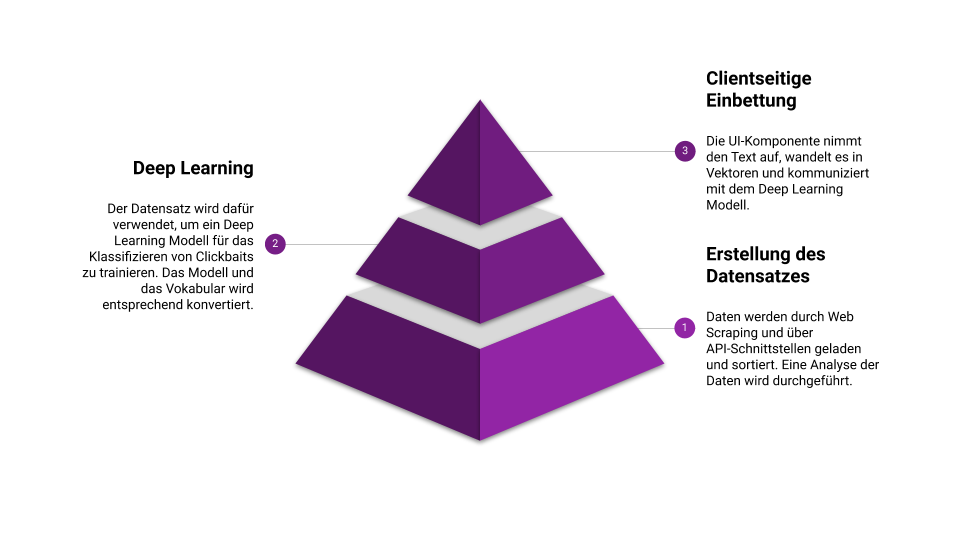
\includegraphics[width=15cm]{kapitel5/main_p.png}
    \caption[Darstellung der Konzeption]{Darstellung der Konzeption}
    \label{Kap5:Konzeption}
\end{figure}


Deep Learning Modelle benötigen eine große Menge an Beispielen um zu lernen. Es reicht außerdem nicht aus, nur eine große Menge an Daten zu beschaffen, sondern auch gute Daten auszuwählen. In der Studie von \cite*{Chakrabortya} haben die Autoren Daten aus dem Web geladen. Für die erste Kategorie, der Nicht-Clickbaits, wurde die Wikipedia-News-API verwendet. Um genug Beispiele für Clickbaits zu finden, sollten solche Medien herausgefunden werden. Um die Daten labeln zu können ist neben dem Titel eines Datenelementes auch die extraktion der Nachricht zu erfassen.

Die Wikipedia-News-API bietet einen Kostenlosen Endpunkt an, welches verschiedene Nachrichtenportale wie z.B. Politik, Wirtschaft, Kultur, Sport und Wissenschaft anbietet. Um Clickbaits zu finden verläuft die Datenaquise wesentlich schwieriger. Der Datensatz von \cite*{Chakrabortya} beinhalter jeweils 7500 Nachrichten je Kategorie. Es ist zu berücksichtigen, dass diese nicht mit Deep Learning Modellen arbeiten, sondern mit klassischen Machine Learning Algorithmen, die weniger Daten benötigen. Es müssen also mehr Daten her, also die Suche sollte neben den klassischen Clickbait-Seiten auch woanders erfolgen. Um die Datenextraktion zu automatisieren bietet sich die Software \enquote{Scrapy} an. Scrapy ist ein Open-Source Tool, welches das extrahieren von großen Mengen an Daten erleichtert. Es ist in Python geschrieben und kann durch seine Middleware Funktion auch die Daten direkt in eine SQL-Datenbank speichern.

Der mittlere Kern der Pyramide in Abbildung~\ref{Kap5:Konzeption} ist das Deep Learning Modell, welches als Inferenzmaschine betrachtet werden kann. Es wird durch Eingabe von gelabelten Daten trainiert und in ein entsprechendes Format gebracht. Es gibt mehrere Anbieter für das Deep Learning. Die meisten von Ihnen sind Open Source. Die bekanntesten Bibliotheken für das Deep Learning sind TensorFlow (welches von Google unterstützt wird) und PyTorch (welches von Facebook unterstützt wird). Seit März 2018 bietet TensorFlow die Möglichkeit, Modelle in der Programmiersprache JavaScript zu trainieren und zu benutzen. Ein klassischer Vorgang um Deep Learning Modelle dem Endbenutzer durch Webprogrammierung anzubieten war es immer, dass zunächst ein Modell trainiert wurde und dann auf einem Server geladen wurde. Der Server hatte dann einen Endpunkt, z.B. eine POST-Anfrage, welches eine Anfrage vom Clienten empfang. Diese Anfrage wurde dann im Server durch das Modell beantwortet und der Server sendete dem Clienten das Ergebnis. Durch TensorFlow.js ist es möglich erstens ein Modell komplett auf der Programmiersprache JavaScript zu entwickeln und zweitens es die Inferenzbildung durch einen Server in der Mitte nicht mehr nötig. Das Modell kann zusammen mit dem Framework in den Browser geladen werden und die bearbeitung erfolgt dort. In dieser Arbeit wurde das Modell nicht mit TensorFlow.js trainiert, da es auch möglich ist, Modelle in der konventionellen Weise mit der Keras API zu trainieren und dann in ein Webfreundliches Format umzuwandeln. Nach der Konversion können die Gewichte welches das Modell gerechnet hat und eine JSON-Datei, welches das Modell beschreibt hochgeladen und benutzt werden. Der Client muss nur noch diese Dateien in den Browser laden und kann dann selbst die Anfrage beantworten. Das trainieren auf konventionellen Wegen bietet außerdem den Vorteil, dass die Umgebung auf JavaScript nicht mit der Umgebung in Python konkurrieren kann. Die meisten Tools und Frameworks werden für Python geschrieben. Ein weiterer Grund ist, dass die bearbeitung auf dem heimischen Computer sehr langsam ist. Mit Google Colab können Deep Learning Modelle mit viel Rechnerkapazität trainiert werden.

Die Spitze der Pyramide macht die Benutzeroberfläsche aus. Diese wird komplett in JavaScript geschrieben. JavaScript ist die meistbenutze Programmiersprache und wird heute neben Webentwicklung auch auf dem Server verwendet. Mit TensorFlow.js ist es nun auch möglich, mit Tensors umzugehen. Die Schwierigkeit hier ist es, den Text, den der Benutzer eingibt, in Token und dann diese Token in Vektoren umzuwandeln, wenn das Modell keinen sogenannten \enquote{Input-Layer} hat welches einfache String einnehmen kann und diese umwandeln kann, dieses macht das Modell aber viel größer, da es eine größere Anzahl an Parametern hat und nicht Ziel dieser Arbeit. Eine andere Möglichkeit ist es, das gesamte Vokabular in einer JSON-Datei zu speichern und es der Benutzeroberfläsche zugänglich zu machen. Jedes auftauchende Wort im Vokabular bekommt einen Index, welches dann als \enquote{Übersetzer} dient und zur Umwandlung der Strings in Vektoren verwendet werden.




\section{Erstellung des Datensatzes}
\subsection{Erste Rohdatenbeschaffung durch Web Scraping}

Um einen Forschungsbeitrag zu leisten, hat diese Arbeit das Ziel ein Clickbait Corpus auf deutscher Sprache zu erstellen. Für die Erstellung eines solchen Korpus sind zunächst bestimmte Seiten einzugrenzen, die Clickbait Nachrichten anbieten. Die bekannteste Seite ist \enquote{buzzfeed} und \enquote{tasty}. Außerdem wurden auch Webseiten wie \enquote{web.de} oder \enquote{tv-movie}\footnote{Beinhaltet außerdem Schlagzeilen aus den Bereichen \enquote{tasty} und \enquote{quiz}} nach Clickbaits gescannt. Das Screening wurde am November 2020 durchgeführt. Um jedoch zu gewährleisten, dass die Nachrichten zeitlich weit außereinder liegen und somit eine größere Diversität haben, wurden Webseiten ausgewählt die Ihre Nachrichten in gewisser Weise Archivieren. Die gesammelten Daten reichen teilweise über ein Jahr zurück. Wie im Listing~\ref{Scrapy} unter in Zeile 12 zu sehen ist, besitzt die Seite im Beispiel eine Pagination-Funktion. Diese kann dafür verwendet werden, um auch ältere Nachrichten zu erfassen.

\begin{table}[h]
    \caption{Vergleich der Rohdaten nach dem Scrapingvorgang}
    \label{Datensatz_Herkunft}
    \renewcommand{\arraystretch}{1.2}
    \centering
    \sffamily
    \begin{footnotesize}
        \begin{tabular}{l l l}
            \toprule
            \textbf{Quelle}   & \textbf{Methodik} & Elemente \\
            \midrule
            de.wikinews.org   & API-Zugang        & 10.612   \\
            web.de            & Web Scraping      & 14.163   \\
            tvmovie.de        & Web Scraping      & 9.428    \\
            buzzfeed.de       & Web Scraping      & 798      \\
            promipool.de      & Web Scraping      & 26.779   \\
            heftig.de         & Web Scraping      & 605      \\
            frauenseite.net   & Web Scraping      & 148      \\
            bravo.de          & Web Scraping      & 7.476    \\
            \midrule
            Summe Clickbaits  &                   & 59.407   \\
            Summe Nachrichten &                   & 10.612   \\
            Summe insgesamt   &                   & 70.019   \\
            \bottomrule
        \end{tabular}
    \end{footnotesize}
    \rmfamily
\end{table}



Das Verfahren wurde automatisch mittels eines programmierten Scrapers je Seite durchgeführt. Ein Scraper ist ein Programm, welches Informationen aus einer Webseite automatisch extrahieren kann. Dieses gelingt, indem es nach HTML- oder CSS-Attributen oder sogar AJAX-Requests durchsucht oder diese imitiert. Im Listing~\ref{Scrapy} wird ein Web-Scraper vorgestellt. Scrapy führt in einer Schleife HTTP-Requests durch welche jeweils eine Antwort bekommen. Es können auch AJAX-Anfragen gesendet werden (z.B. ein POST-Request). Wenn die Anfrage Erfolgreich ist, kann die daraus resultierende Antwort auf bestimmte Eigenschaften und Attribute durchsucht werden (im Beispiel werden CSS-Attribute durchsucht). Diese Attribute beinhalten meisten die gewünschte Information, welches dann wie in der \texttt{parse\_url} und \texttt{parse\_page} Methode gezogen und in eine Datenbank gespeichert wird.



\begin{lstlisting}[language=Python,caption=Beispiel eines Scrapers]
import scrapy
from scrapy.http.request import Request
from datetime import datetime
from klickscraper.items import WebdeItem


class WebdeSpider(scrapy.Spider):
    name = "webde"
    scraped_at = datetime.now()

    def start_requests(self):
        for i in range(287):
            url = f"https://web.de/magazine/unterhaltung/stars/p{i}"
            yield Request(
                dont_filter=True,
                callback=self.parse_url,
                url=url)

    def parse_url(self, response):
        follow_ulrs = response.css(
            ".teaser-article__full").css("a::attr(href)").getall()
        for f in follow_ulrs:
            yield Request(
                url=f,
                dont_filter=True,
                callback=self.parse_page)

    def parse_page(self, response):
        if len(response.css("p::text").getall()) > 10:
            text = " ".join(response.css("p::text").getall())
        else:
            text = None
        yield WebdeItem(title=response.css('title::text').get(),
                        text=text,
                        scraped_at=self.scraped_at)
\end{lstlisting}\label{Scrapy}


\subsection{Explorative Datenanalyse der Rohdaten}
Um aus den Rohdaten Schlüsse über die sprachlichen Eigenschaften zu ziehen wird im folgenden Abschnitt eine explorative Datenanalyse durchgeführt. Um dies möglichst zu vereinfachen, wird der Rohdatensatz welches in einer SQL-Datenbank gespeichert wurde in ein Pandas\footnote{Pandas ist ein schnelles, flexibles und benutzerfreundliches Open-Source-Tool zur Analyse und Bearbeitung von Daten in Python.} Dataframe umgewandelt.
Aus der Abbildung~ist zu sehen, dass die Titel aus Wikinews länger sind. Neben der Länge der Schlagzeilen ist auch die Analyse der Wortauswahl wichtig. Aus der Literaturstudie können bestimmte Merkmale von Clickbaits festgestellt werden. Clickbaits enthalten meistens eine Frage oder Zahlen. Außerdem ist bei Clickbaits auch eine gewisse Wortauswahl festzustellen. Die Zuordnung der Wörter je Clickbait-Schlagzeile zu den Wortarten (Part-of-speech-Tagging oder POS-Tagging) wurde mittels der Python NLP-Bibliothek Spacy durchgeführt. Bei der Auswahl der Tags nachdem gesucht werden sollte, wurden die Erkenntnisse aus Kapitel 4 Berücksichtigt. Die Ergebnisse diese Analyse sind aus der Tabelle~\ref{pos} zu entnehmen.

\begin{table}[h]
    \caption{Vergleich der Ergebnisse des Part-of-speech-Taggings}
    \label{pos}
    \renewcommand{\arraystretch}{1.2}
    \centering
    \sffamily
    \begin{footnotesize}
        \begin{tabular}{l l l}
            \toprule
            \textbf{TAG}                  & \textbf{Auffälliges Wort (Häufigkeit)} \\
            \midrule
            ADJA  (attributives Adjektiv) & neu (1759), neue (1474)                \\
            ADJD   (adverbiales Adjektiv) & krass (171), wirklich  (349)           \\
            ADV   (Adverb)                & so (5142), endlich (357)               \\
            PDAT (Demonstrativpronomen)   & dies (3566)                            \\
            PROAV   (Pronominaladverb)    & darum (588), deshalb (251)             \\
            PWAT (Interrogativpronomen)   & welch (154)                            \\
            PWAV  (Relativpronomen)       & wie (488) warum (184)                  \\
            \bottomrule
        \end{tabular}
    \end{footnotesize}
    \rmfamily
\end{table}

% Eine eigene Analyse durch das Part-of-Speech_tagging mittels Scrapy ergibt einige Auffälligkeiten bezüglich der Clickbaits. Wörter wie \enquote{diese} (attribuierendes Demonstratives Pronomen), \enquote{warum} (adverbiales Interrogativ- oder Relativpronomen) oder \enquote{welche} (attribuierendes Interrogativpronomen) sind einige Auffällige Tags aus den Schlagzeilen der Clickbaits.



% \begin{lstlisting}[language=Python,caption=Funktion zur Umwandung der Datenbank in en Pandas Dataframe]
% def connect_to_db(tablename, db_path):
%     return pd.read_sql_query(
%         f"SELECT * FROM {tablename}", sqlite3.connect(db_path))
% \end{lstlisting}\label{Pandasdb}


\begin{figure}[H]
    \centering
    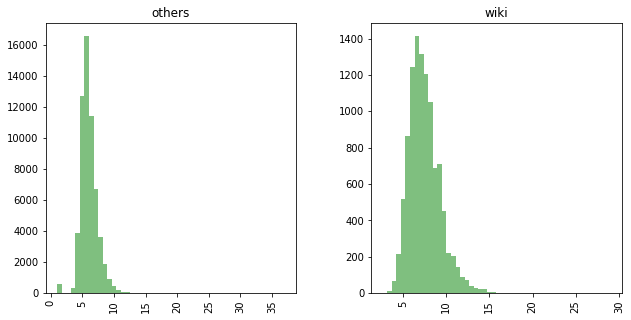
\includegraphics[width=14cm]{kapitel5/hist2.png}
    \caption[Vergleich der Wortlängen der Rohdaten]{Vergleich der Wortlängen, das Histogramm rechts (Wikinews) ist breiter als das Histogramm links (Clickbaits)}
    \label{Kap5:Hist2}
\end{figure}

% \begin{figure}[H]
%     \centering
%     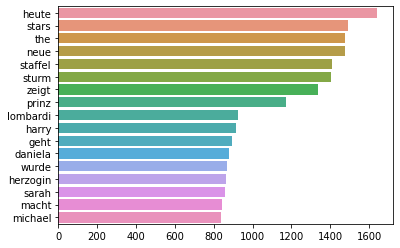
\includegraphics[width=10cm]{kapitel5/freq_word1.png}
%     \caption[Häufigsten Wörter aus den Rohdaten der Clickbaits Titel]{Die Darstellung zeigt das Aufkommen der Häufigsten Wörter aus den Titeln der Clickbaits}
%     \label{Kap5:freq1}
% \end{figure}

% \begin{figure}[H]
%     \centering
%     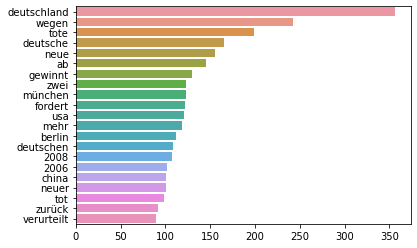
\includegraphics[width=10cm]{kapitel5/freq_word2.png}
%     \caption[Häufigsten Wörter aus den Rohdaten der Wikinews Titel]{Die Darstellung zeigt das Aufkommen der Häufigsten Wörter aus den Titeln der Wikinews Nachrichten}
%     \label{Kap5:freq2}
% \end{figure}


\subsection{Labeln der Daten}
Aus der Tabelle~\ref{Datensatz_Herkunft} ist zu entnehmen, dass ca. 60.000 potenzielle Clickbaits vorhanden sind. Um dieses nicht per Hand labeln zu müssen besteht der Ansatz darin, bestimmte Muster zu erkennen und diese Muster auszunutzen, um die Anzahl der Kandidaten auf ein entsprechendes niedriges Niveau zu bringen. Die Literaturstudie und die explorative Datenanalyse bringen gemeinsam folgende Schlüsse:

\begin{enumerate}
    \item Clickbaits sind meisten Fragen wie \enquote{Welcher Schuh passt dir am meisten?}
    \item Clickbaits enthalten meistens Zahlen in Form eines Listings \enquote{Das sind die 10 schnellsten Autos}
    \item Clickbaits haben eine niedrigere Wortlänge als normale Nachrichten
    \item Clickbaits beinhalten einige für sie markanten Wörter wie \enquote{diese} oder \enquote{so}
\end{enumerate}

Diese Erkenntnisse können programmatisch umgewandelt werden und somit der Rohdatensatz um ein vielfaches reduziert werden.


\begin{lstlisting}[language=Python,caption=Funktion welches ein Dataframe je nach Argumenten labelt]
def contains_word(word, row):
    for r in row:
        if r in word:
            return 1


def label_data_with_arg(df, col_name, arg_):
    return df[col_name].apply(
        lambda x: contains_word(arg_, re.findall(r"[\w']+|[.,!?;]", x.lower())))
\end{lstlisting}\label{Label1}

\begin{lstlisting}[language=Python,caption=Funktionen für durchschnittliche Wortlänge und Interpunktion]
import re
import string

def remove_punc(text):
    text = re.sub('\[.*?\]', '', text)
    text = re.sub('https?://\S+|www\.\S+', '', text)
    text = re.sub('<.*?>+', '', text)
    text = re.sub('[%s]' % re.escape(string.punctuation), '', text)
    text = re.sub('\n', '', text)
    text = re.sub('\w*\d\w*', '', text)
    return text

def get_avg_length(string):
    words = remove_punc(string).split()
    try:
        count = int(sum(len(word) for word in words) / len(words))
    except ZeroDivisionError:
        count = 1
    return count
\end{lstlisting}\label{Label2}

\begin{lstlisting}[language=Python,caption=Tagger Funktion]
import spacy
nlp = spacy.load('de')

def contains_pos(sentence):
    list_ = ["PDAT", "ADJD", "ADJA", "PIS", "PWAV", 
            "PTKA", "VAFIN", "PROAV", "ADV"]
    doc = nlp(sentence)
    for token in doc:
        if str(token.tag_) in list_:
            return "1"

def label_data_with_pos(df, col_name):
    return df[col_name].apply(
        lambda x: contains_pos(x.lower()))
\end{lstlisting}\label{Label3}


\subsection{Analyse der Daten}
Die Summe der Wikinews Nachrichten beträgt ca. 10.000. Mit der Zugabe weiterer 10.000 Clickbaits, die durch das labeln entstehen, ergibt sich ein Datensatz mit 20.000 Beispielen. Die Tabelle~\ref{data} verschafft einen Übrerblick über alle Daten. Interessant ist bei den Clickbaits, dass ca. 33\% aller Clickbaits ein Fragezeichen oder eine Zahl beinhalten und ca. die hälfte aller Daten im Datensatz ein bestimmtes Tag wie \enquote{diese} oder \enquote{so} enthalten. Bei den Wikinews Nachrichten liegen diese Anteile deutlich unten. Alle drei genannten Eigenschaften liegen unter 1\%. Die durchscnittliche Wortlänge beträgt bei den Clickbaits bei 5, während bei den Wikipedia Nachrichten dieses bei 7 liegt.

\begin{table}[h]
    \caption{Beschreibung des gelabelten Datensatzes}
    \label{data}
    \renewcommand{\arraystretch}{1.2}
    \centering
    \sffamily
    \begin{footnotesize}
        \begin{tabular}{l l l l l l}
            \toprule
                           & \textbf{has\_question} & \textbf{has\_keyword} & \textbf{has\_number} & \textbf{avg\_word\_length} & \textbf{label} \\
            \textbf{count} & 20000                  & 20000                 & 20000                & 20000                      & 20000          \\
            \textbf{mean}  & 0.1782                 & 0.3190                & 0.0854               & 6.1307                     & 0.5000         \\
            \textbf{std}   & 0.3826                 & 0.4661                & 0.2795               & 1.7874                     & 0.5000         \\
            \textbf{min}   & 0                      & 0                     & 0                    & 1.0000                     & 0              \\
            \textbf{max}   & 1                      & 1                     & 1                    & 27.0000                    & 1              \\

            \bottomrule
        \end{tabular}
    \end{footnotesize}
    \rmfamily
\end{table}

Bei der Betrachtung der Wörter mit der Word-Cloud Analyse können bestimmte Themen, die die Titel zürückgeben betrachtet werden.  Auffällig sind neben Promis auch die Wörter \enquote{darum}, \enquote{quiz} \enquote{sieht} und \enquote{macht}. Bei den Wikipedia Nachrichten geht es mehr um Deutschland und der Welt.


\begin{figure}[H]
    \centering
    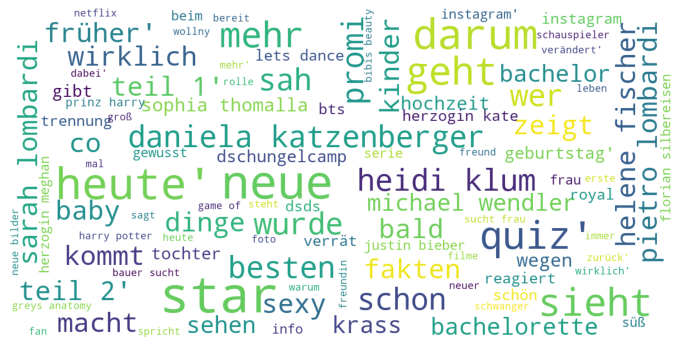
\includegraphics[width=12cm]{kapitel5/wo_click.png}
    \caption[Word Cloud Analyse für die Clickbaits Schlagzeilen]{Die Darstellung zeigt das Aufkommen der Häufigsten Wörter aus den Titeln der Wikinews Nachrichten}
    \label{Kap5:clwc}
\end{figure}

\begin{figure}[H]
    \centering
    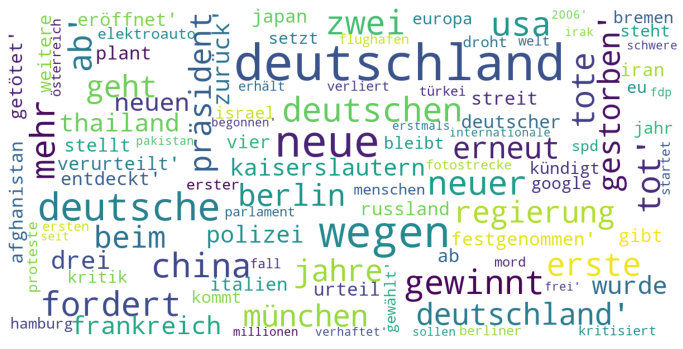
\includegraphics[width=12cm]{kapitel5/news.png}
    \caption[Word Cloud Analyse für die Wikinews Schlagzeilen]{Die Darstellung zeigt das Aufkommen der Häufigsten Wörter aus den Titeln der Wikinews Nachrichten}
    \label{Kap5:clwc}
\end{figure}


\section{Das Deep Learning Modell}
\subsection{Einleitung}
\subsection{Soft- und Hardware}
\textit{TensorFlow} ist eine Bibliothek, mit der Deep Learning durchgeführt werden können, es wurde im Jahr 2015 von Google Open Source gemacht. Mit TensorFlow werden die Datan als Tensoren dargestellt und fließen durch Schichten. Dieses ermöglicht die Inferent und das Traiing in maschinellen Lernmodellen. Ein Tensor ist ein multidimensionales Array. In neuronalen Netzen und beim Deep Learning wird jedes Datenelement und jedes Berechnungsergebnis als Tensor dargestellt, z.B. kann ein Graustufenbild als 2-Dimensionales-Array dargstellt werden oder ein Farbbild als 3-Dimensionales-Array. Der Tensor kann unterschiedliche Datentypen haben (z. B. float32 oder int32). Neben dem Typen eines Tensors gibt es die zweite Eigenschaft, die Form eines Tensors. Die Form eines Tensors gibt die Größe des Tensors entlang aller seiner Abmessungen an. Beispiel: Ein 2-Dimensionales-Tensor hat die Form (128, 256). Ein Tensor kann unabhängig von den ursprünglichen Daten in ein sogenanntes Layer eingespeist werden, welches nur danach schaut, welcher Datentyp und Form der Tensor hat. Tensoren sind also eine Art Container die Daten organisieren und dafür verwendet werden können, dass diese parallel verarbeitet werden können.


\begin{lstlisting}[language=Python,caption=Beispiel eines Tensors in TensorFlow]
import tensorflow as tf
rank_2_tensor = tf.constant([[1, 2],
                             [3, 4],
                             [5, 6]], dtype=tf.float16)
\end{lstlisting}\label{Label3}

Um den zweiten Ausdruck in \enquote{TensorFlow} zu verstehen muss der Tensor als eine Art \enquote{Flüssigkeit} vorgestellt werden, welches die Daten trägt. In TensorFlow fließt es durch ein Diagramm - eine Datenstruktur, die aus miteinander verbundenen mathematischen Operationen (Knoten genannt) besteht. Wie Abbildung~\ref{tnflayers} zeigt, kann der Knoten aufeinanderfolgende Schichten in einem neuronalen Netzwerk sein. Jeder Knoten nimmt Tensoren als Eingaben und erzeugt Tensoren als Ausgaben. Die \enquote{Flüssigkeit} wird in verschiedene Formen und Werte umgewandelt, wenn sie durch das TensorFlow-Diagramm \enquote{fließt}. Dies entspricht der Transformation von, d.h. dem Kern dessen, was neuronale Netze tun. Mit TensorFlow können Ingenieure für maschinelles Lernen alle Arten von neuronalen Netzen schreiben, von flachen bis zu sehr tiefen, von CNN für Computer Vision bis zu wiederkehrenden neuronalen Netzen (RNNs) für Sequenzaufgaben .

 \begin{figure}[H]
     \centering
     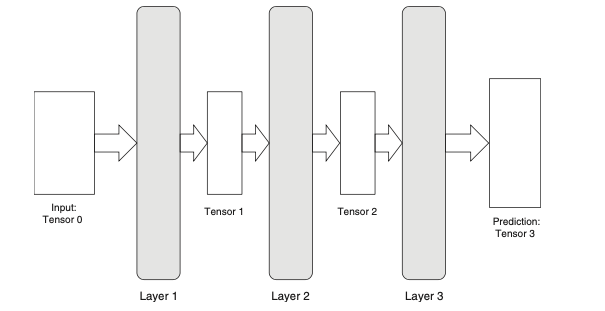
\includegraphics[width=10cm]{kapitel5/tflayers.png}
     \caption[Die Darstellung eines Deep Learning Modells in Tensorflow]{Die Darstellung eines Deep Learning Modells in Tensorflow - Die Tensoren fließen durch jede Schciht im Modell durch (Abbildung aus)}
     \label{Kap5:tnflayers}
 \end{figure}


Im Kern wurde TensorFlow sehr allgemein und flexibel konzipiert: Die Operationen können beliebige genau definierte mathematische Funktionen sein, nicht nur Schichten neuronaler Netze. Dies können beispielsweise mathematische Operationen auf niedriger Ebene sein, beispielsweise das Addieren und Multiplizieren von zwei Tensoren - die Art von Operationen, die innerhalb einer neuronalen Netzwerkschicht stattfinden. Dies gibt Deep-Learning-Ingenieuren und -Forschern die Möglichkeit, beliebige und neuartige Operationen für Deep-Learning zu definieren. Für einen großen Teil der Deep-Learning-Praktiker ist die Manipulation solcher Maschinen auf niedriger Ebene jedoch schwieriger als es sich lohnt. Dies führt zu aufgeblähtem und fehleranfälligerem Code und längeren Entwicklungszyklen. Die meisten Deep-Learning-Ingenieure verwenden eine Handvoll fester Schichttypen (z. B. Faltung, Pooling oder Dichte). In seltenen Fällen müssen neue Ebenentypen erstellt werden. Hier ist die LEGO-Analogie angebracht. Bei LEGOs gibt es nur wenige Blocktypen. LEGO Builder müssen nicht darüber nachdenken, was nötig ist, um einen LEGO Block zu erstellen. Dies unterscheidet sich von einem Spielzeug wie beispielsweise Play-Doh, das der Low-Level-API von TensorFlow entspricht.

Die Fähigkeit, LEGO-Blöcke zu verbinden, führt jedoch zu einer kombinatorisch großen Anzahl von Möglichkeiten und einer praktisch unendlichen Leistung. Es ist möglich, ein Spielzeughaus mit LEGOs oder Play-Doh zu bauen. Wenn Sie jedoch keine besonderen Anforderungen an Größe, Form, Textur oder Material des Hauses haben, ist es viel einfacher und schneller, es mit LEGOs zu bauen. Für die meisten von uns wird das LEGO-Haus, das wir bauen, stabiler stehen und schöner aussehen als das Play-Doh-Haus, das wir bauen würden.

In der Welt von TensorFlow ist das LEGO-Äquivalent die High-Level-API namens Keras.  Keras bietet eine Reihe der am häufigsten verwendeten Arten von neuronalen Netzwerkschichten mit jeweils konfigurierbaren Parametern. Außerdem können Benutzer die Schichten miteinander verbinden, um neuronale Netze zu bilden. Darüber hinaus enthält Keras auch APIs für

\begin{itemize}
     \item Festlegen, wie das neuronale Netzwerk trainiert werden soll (Verlustfunktionen, Metriken und Optimierer)
     \item Daten einspeisen, um das neuronale Netzwerk zu trainieren oder auszuwerten oder das Modell zur Inferenz zu verwenden
     \item Überwachung des laufenden Schulungsprozesses (Rückrufe)
     \item Modelle speichern und laden
     \item Drucken oder Plotten der Architektur von Modellen
 \end{itemize}



Mit Keras können Benutzer den gesamten Deep-Learning-Workflow mit sehr wenigen Codezeilen ausführen. Mit der Flexibilität der Low-Level-API und der Verwendbarkeit der High-Level-API bilden TensorFlow und Keras ein Ökosystem, das im Bereich der Deep-Learning-Rahmenbedingungen hinsichtlich der industriellen und akademischen Akzeptanz führend ist. Als Teil der anhaltenden Deep-Learning-Revolution sollte ihre Rolle, Deep Learning einem breiteren Publikum zugänglich zu machen, nicht unterschätzt werden. Vor Frameworks wie TensorFlow und Keras konnten nur diejenigen mit CUDA-Programmierkenntnissen und umfassender Erfahrung im Schreiben neuronaler Netze in C++ praktisches Deep Learning durchführen. Mit TensorFlow und Keras ist es viel weniger erforderlich, GPU-beschleunigte tiefe neuronale Netze zu erstellen.

Es gab jedoch ein Problem: Es war nicht möglich, TensorFlow- oder Keras-Modelle in JavaScript oder direkt im Webbrowser auszuführen. Um Deep-Learning-Modelle im Browser bereitzustellen, musste dies über HTTP-Requests an einen Backend-Server getan werden. TensorFlow.js löst dieses Problem. Die JavaScript-API hat eine Keras-ähnliche High-Level-API welches auf dem Low-Level-Kern erstellt wurde, die es Benutzern erheblich erleichtert, Deep-Learning-Modelle in der JavaScript-Bibliothek zu definieren, zu trainieren und auszuführen. Um die Interoperabilität weiter zu verbessern, wurden Konverter erstellt, mit denen TensorFlow.js aus TensorFlow und Keras gespeicherte Modelle importieren und Modelle in diese exportieren kann.

 \begin{figure}[H]
     \centering
     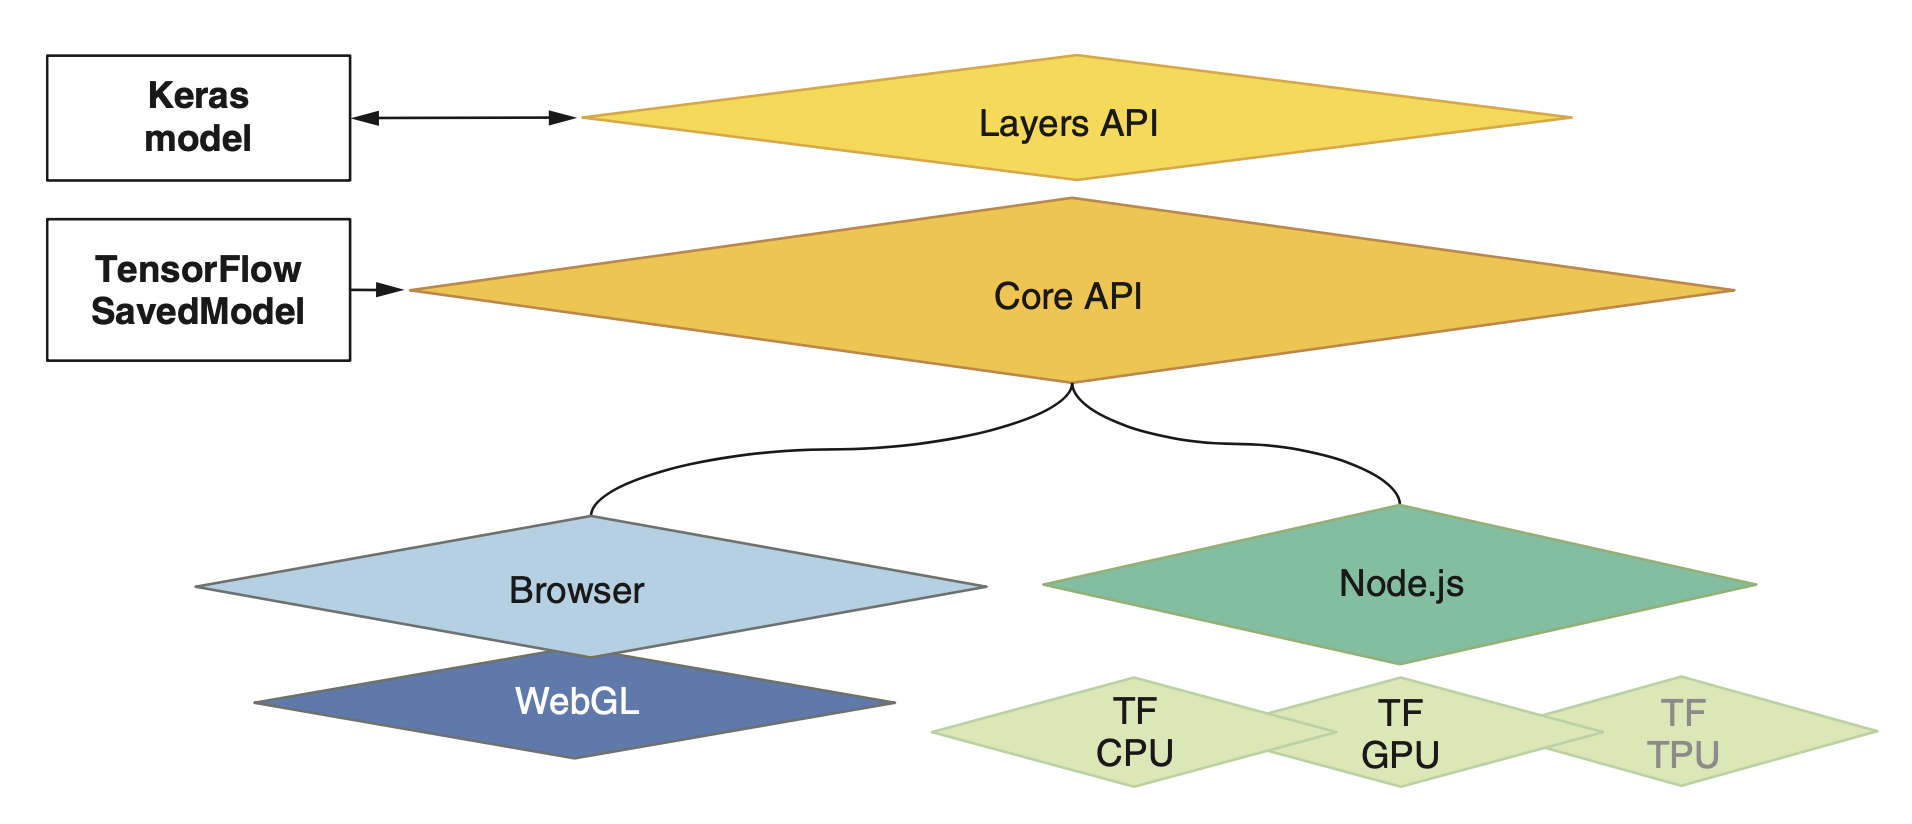
\includegraphics[width=12cm]{kapitel5/tfjsarch.png}
     \caption[Die Architektur von TensorFlow.js]{Die Architektur von TensorFlow.js - Abbildung zeigt die Verhältnisse zwischen der Paython API von TensorFlow und Keras mit TensorFlow.js}
     \label{Kap5:tfjsarch}
 \end{figure}

\subsection{Preporcessing}
\subsection{Tokenisierung}
\subsection{Embedding Layer}
\subsection{Das CNN-Model}
\subsection{Training und Evaluation}
\subsection{Umwandlung und Export in ein Webformat}
%(mit Vocab.json)
\subsection{Schluss}

















\appendix 
\chapter{Anhang}
\label{chapter:Anhang}









\clearpage
        \phantomsection % damit das pdf bookmark an die richtige Stelle zeigt
        \pdfbookmark{Literaturverzeichnis}{bibliography}
        
        % zeigt immer alle definierten Quellen an, auch wenn diese nicht verwendet werden
        %\nocite{*}
        \bibliographystyle{abbrv}
        \addcontentsline{toc}{chapter}{Literaturverzeichnis}
        \bibliography{literatur}




\chapter*{Erklärung}
Hiermit versichere ich, dass ich die vorliegende Arbeit selbstständig verfasst und keine anderen als die angegebenen Quellen und Hilfsmittel benutzt habe, insbesondere keine anderen als die angegebenen Informationen aus dem Internet. Diejenigen Paragraphen der für mich gültigen Prüfungsordnung, welche etwaige Betrugsversuche betreffen, habe ich zur Kenntnis genommen. Der Speicherung meiner Projekt-Arbeit zum Zweck der Plagiatsprüfung stimme ich zu. Ich versichere, dass die elektronische Version mit der gedruckten Version inhaltlich übereinstimmt.\newline
\linebreak
\linebreak
\linebreak
Bielefeld, den \today\newline
(Ort) (Datum)\newline
\linebreak
\linebreak
\linebreak
..................................\newline
(Unterschrift)
\end{document}